\documentclass[12pt,a4paper]{report}

\usepackage[utf8]{inputenc}
\usepackage[T1]{fontenc}
\usepackage{geometry}
\geometry{top=20mm, bottom=20mm, left=25mm, right=20mm}
\usepackage{amsmath,amssymb,amsfonts}
\usepackage{graphicx}
\usepackage{booktabs}
\usepackage{tabularx}
\usepackage{multirow}
\usepackage{hyperref}
\hypersetup{
    colorlinks=true,
    linkcolor=blue,
    citecolor=blue,
    urlcolor=cyan,
    pdftitle={Soft Robotic Grippers using Tactile Sensor},
    pdfauthor={G. Chandana, Shinde Sanchali Sanjay, Saurav Shekhar}
}
\usepackage{fancyhdr}
\pagestyle{fancy}
\fancyhf{}
\fancyhead[L]{\small\nouppercase{\leftmark}}
\fancyhead[R]{\small\thepage}
\renewcommand{\headrulewidth}{0.4pt}
\usepackage{setspace}
\onehalfspacing
\usepackage{cite}
\usepackage{caption}
\usepackage{subcaption}

\begin{document}

% ==================== TITLE PAGE (EXACT PROFESSOR FORMAT) ====================
\begin{titlepage}
\centering
\vspace*{-5mm}
\fbox{\begin{minipage}[c][0.93\textheight][c]{0.93\textwidth}
\centering
\vspace{6mm}
{\LARGE \textbf{Soft Robotic Grippers using Tactile Sensor}\par}
\vspace{16mm}
{\large Report submitted to\par}
\vspace{2mm}
{\Large \textbf{Indian Institute of Technology, Kharagpur}\par}
\vspace{2mm}
{\large For the fulfillment of BTP-I in\par}
\vspace{14mm}
{\large \textit{Mechanical Engineering with specialisation in}\par}
\vspace{1mm}
{\large \textit{Manufacturing Science and Engineering by}\par}
\vspace{14mm}
{\large \textbf{G. Chandana (23ME31008)}\par}
\vspace{2mm}
{\large \textbf{Shinde Sanchali Sanjay (23ME31029)}\par}
\vspace{2mm}
{\large \textbf{Saurav Shekhar (23ME31043)}\par}
\vspace{14mm}
{\large Under the\par}
\vspace{2mm}
{\large Supervision of\par}
\vspace{2mm}
{\Large \textbf{Prof. Sankha Deb}\par}
\vspace{8mm}

\includegraphics[width=46mm]{../Figures and Diagrams/iitkgp_logo.png}\par
\vspace{10mm}
{\Large \textbf{Department of Mechanical Engineering}\par}
\vspace{2mm}
{\Large \textbf{Indian Institute of Technology, Kharagpur - 721302}\par}
\vspace{4mm}
\end{minipage}}
\end{titlepage}

\newpage
\pagenumbering{roman}
\setcounter{page}{2}

\chapter*{Certificate of Approval}
\addcontentsline{toc}{chapter}{Certificate of Approval}
This is to certify that the project report entitled \textbf{``Development, Non-linear Modeling, and Embedded Tactile Control of a 3D-Printed Compliant Soft Robotic Gripper''} submitted by \textbf{G. Chandana} (23ME31008), \textbf{Shinde Sanchali Sanjay} (23ME31029), and \textbf{Saurav Shekhar} (23ME31043) to the Indian Institute of Technology Kharagpur, for the partial fulfillment of the requirements for the award of the degree of Bachelor of Technology in Mechanical Engineering (with specialization in Manufacturing Science and Engineering), is a bona fide record of the work carried out by them under my supervision and guidance.

The project is currently at the literature-review-completed stage, and the proposed methodology, numerical simulation framework, and experimental implementation roadmap have been thoroughly examined and approved for progression into Project Stage-II (BTP-II).

\vspace{30mm}
\noindent
\begin{tabular}{@{}p{80mm}p{70mm}@{}}
\textbf{Prof. Sankha Deb} & \textbf{Date:} November 2026 \\
Supervisor & \textbf{Place:} IIT Kharagpur \\
Department of Mechanical Engineering & \\
Indian Institute of Technology, Kharagpur & \\
\end{tabular}

% ==================== ABSTRACT ====================
\newpage
\chapter*{Abstract}
\addcontentsline{toc}{chapter}{Abstract}
Traditional robotic manipulation systems rely on rigid articulated linkages that exhibit high positioning repeatability but lack intrinsic compliance, rendering them prone to crushing delicate, fragile, or irregularly contoured objects in automated agriculture, biomedical packaging, and explosive ordnance handling. Soft robotic end-effectors address this limitation through structural deformability, enabling passive geometric conformity and safe contact pressure distribution. However, conventional soft grippers suffer from severe engineering bottlenecks: low payload capacity, material hysteresis, complex tethered fluidic supplies, sensor-skin delamination, and an absence of localized feedback capable of detecting incipient slip without bulky optical apparati.

This report establishes the complete Stage-I research foundation and detailed Stage-II implementation roadmap for a \textbf{Monolithic 3D-Printed (FDM TPU) Tendon-Driven Compliant Soft Robotic Gripper with Embedded Tactile Sensing}. Synthesizing an extensive multi-author literature corpus, the research evaluates fluidic elastomer actuators (PneuNets), shape memory alloys (Nitinol), and cable-driven compliant architectures. To overcome mold-tooling delays and fluid leakage risks, a direct additive manufacturing route using Thermoplastic Polyurethane (TPU 95A) is formulated, integrating circular flexure living hinges that eliminate mechanical joint backlash while maximizing structural fatigue life. 

To provide deterministic grasp autonomy, thin-film Force Sensitive Resistors (FSR402) are integrated flush into the phalange contact pads. An integrated mechatronic architecture centered on a dual-core ESP32 executing FreeRTOS is developed. The tactile signal pipeline decouples static normal contact force estimation (via an active second-order low-pass Butterworth filter at $f_c = 20\text{ Hz}$) from dynamic incipient slip micro-vibrations (via a 256-point Fast Fourier Transform analyzing the $100 - 300\text{ Hz}$ spectral energy band). This enables closed-loop servomotor torque compensation in under 35 milliseconds. A non-linear finite element analysis (FEA) framework utilizing Mooney-Rivlin hyperelastic strain energy formulations is established to predict tip deflection and stress concentrations prior to physical fabrication. Finally, a structured 16-week semester roadmap is detailed, establishing quantitative benchmarks for pull-out retention force, payload-to-weight ratio, and an autonomous slip-prevention demonstration on physical hardware.

\vspace{5mm}
\noindent\textbf{Keywords:} Soft Robotics, Compliant Mechanisms, Additive Manufacturing, TPU 95A, Tactile Sensing, FSR402, Fast Fourier Transform, Incipient Slip Detection, FreeRTOS, Hyperelastic FEA.

% ==================== CONTENTS & LISTS ====================
\newpage
\tableofcontents
\newpage
\listoffigures
\newpage
\listoftables

% ==================== CHAPTER 1 ====================
\newpage
\pagenumbering{arabic}
\setcounter{page}{1}

\chapter{Introduction}

\section{Background of Soft Robotics and Compliant Manipulation}
Robotic manipulation systems have traditionally been engineered around rigid mechanical kinematic chains composed of metallic or hard polymeric links joined by discrete revolute, prismatic, or spherical hinges. Such systems achieve sub-millimeter positioning accuracy, high structural rigidity, and substantial load-bearing capacities when operating in structured industrial environments where target workpieces possess invariant dimensions, known orientations, and high mechanical stiffness.

However, modern automation requirements are rapidly shifting toward unstructured and semi-structured domains, such as the selective harvesting of fragile agricultural produce (e.g., tomatoes, strawberries, peaches), handling delicate specimens in biomedical logistics, sorting irregular post-consumer recycling items, and conducting hazardous explosive ordnance disposal (EOD). In these settings, traditional rigid end-effectors exhibit intrinsic limitations:
\begin{itemize}
    \item \textbf{Localized Stress Spikes:} Point contacts between rigid jaw faces and fragile objects create severe stress concentrations that exceed the shear or compressive yield strength of delicate cellular or biological structures, leading to bruising, crushing, or structural rupture.
    \item \textbf{High Control Complexity for Sensorless Interaction:} Grasping unknown geometries with rigid multi-jointed fingers demands real-time multi-axis vision tracking, high-order inverse kinematics, and complex active compliance force control.
    \item \textbf{Dynamic Instability and Object Ejection:} Inadequate contact compliance results in microscopic contact chatter and rapid slip transitions if the target shifts during high-speed arm trajectory execution.
\end{itemize}

Soft robotics represents a paradigm shift in end-effector design by replacing rigid links and discrete mechanical pins with continuously deformable elastomeric bodies and monolithic compliant mechanisms \cite{whitesides2018soft, rus2015design}. By embodying \textit{mechanical intelligence} directly into the elasticity of the material, soft grippers passively adapt their morphological shape to envelop complex contours upon contact, distributing interaction forces over an expanded surface area.

\section{Motivation and Industrial Relevance}
The primary motivation for this project stems from the critical need for a low-cost, self-contained, lightweight, and sensorized soft robotic gripper capable of executing delicate manipulation while providing real-time feedback regarding contact force and grasp stability. 

Specific target applications include:
\begin{enumerate}
    \item \textbf{Automated Agricultural Harvesting:} Gentle detachment and transfer of soft-skinned fruits and vegetables without inducing bruised tissue that accelerates biological decay.
    \item \textbf{Biomedical and Pharmaceutical Logistics:} Sorting and transferring thin-walled glass vials, filled fluid ampoules, surgical specimens, and laboratory glassware where mechanical shock must be strictly eliminated.
    \item \textbf{Explosive Ordnance Disposal (EOD):} Interfacing with uncertain, aged, or structurally compromised explosive devices where uncontrolled impact, spark generation, or excessive clamping force could trigger catastrophic detonation.
\end{enumerate}

\section{Research Issues and Technical Challenges}
While the passive adaptability of soft robotics offers clear advantages, it introduces severe engineering trade-offs that do not exist in conventional rigid mechanisms:
\begin{itemize}
    \item \textbf{Non-linear Continuum Mechanics:} Compliant elastomeric structures undergo geometric and material non-linearities under actuation. Standard linear elastic assumptions ($\sigma = E \epsilon$) break down completely under large strains ($>20\%$), demanding non-linear hyperelastic constitutive formulations.
    \item \textbf{Hysteresis and Actuation Lag:} Soft materials dissipate mechanical energy viscoelastically during deformation cycles. The loading and unloading trajectories diverge significantly, reducing open-loop repeatability.
    \item \textbf{Tethering and Portability Limitations:} The vast majority of published soft grippers depend on pneumatic fluidic elastomer actuators (PneuNets). While compliant, they require external compressors, accumulator tanks, proportional regulators, and directional solenoid valves, tethering the end-effector and rendering it impractical for mobile robotic bases.
    \item \textbf{Sensory Blindness and Slip Vulnerability:} Unlike rigid joints fitted with high-resolution digital optical encoders, a continuous soft finger possesses infinite kinematic degrees of freedom. Without tactile sensors, the robot controller cannot ascertain the actual grasp state, resulting in dropped objects when external inertial or gravitational disturbances exceed interfacial friction.
    \item \textbf{Sensor-Actuator Impedance Mismatch:} Integrating thin-film or rigid force sensors into a stretching soft elastomeric skin causes interfacial shear failure, localized stiffening, delamination under repeated bending, and non-linear baseline drift.
\end{itemize}

\section{Broad Objectives of the Present Research}
To resolve these interconnected challenges, this research establishes an integrated mechatronic design combining:
\begin{enumerate}
    \item A \textbf{monolithic 3D-printed compliant finger architecture} fabricated from Thermoplastic Polyurethane (TPU 95A) using direct FDM additive manufacturing, eliminating mold tooling and fluid leakage risks.
    \item An underactuated \textbf{tendon-driven actuation mechanism} placing servomotors remotely on the gripper palm to minimize distal moving mass while maximizing payload-to-weight ratio.
    \item \textbf{Embedded piezoresistive tactile sensing} (FSR402) mounted in recessed, strain-shielded cavities on the finger grasping pads.
    \item An onboard \textbf{dual-core edge processing pipeline} (ESP32 / FreeRTOS) capable of executing high-speed analog filtering for static force tracking alongside real-time Fast Fourier Transform (FFT) spectral analysis for autonomous incipient slip prevention.
\end{enumerate}

% ==================== CHAPTER 2 ====================
\chapter{Literature Review}

\section{Existing National and International Research}
Soft robotics and compliant grasping have witnessed substantial growth over the past decade. Landmark contributions by Whitesides and colleagues \cite{whitesides2018soft, mosadegh2014pneumatic} established fluidic elastomer actuators (PneuNets) as the foundational paradigm for gentle grasping. Subsequent works expanded into dielectric elastomer actuators (DEAs) \cite{shintake2018soft}, shape memory alloys (SMAs) \cite{polygerinos2017soft}, and granular jamming universal end-effectors \cite{rus2015design}. 

In parallel, research in compliant mechanisms, pioneered by Howell \cite{howell2001compliant}, demonstrated that monolithic structures utilizing living hinges can achieve large angular deflections without mechanical assembly, friction, or lubrication requirements. In the domain of tactile perception, Dahiya et al. \cite{dahiya2010tactile} surveyed tactile transduction mechanisms across human biology and robotics, demonstrating that human skin decouples slow-adapting (SA) mechanoreceptors for sustained pressure from fast-adapting (FA) mechanoreceptors for dynamic micro-vibrations and slip.

\section{Synthesis of Available Student Literature Corpus}
The technical literature reviewed by the project team members has been categorized into three specialized thematic domains:
\begin{enumerate}
    \item \textbf{Actuation Schemes and Gripper Architectures (Shinde Sanchali Sanjay) \cite{btp_source_sanchali}:} A systematic evaluation of robotic arm grippers categorized by mechanical mobility, degrees of freedom, and actuation physics (fluidic, tendon, thermal SMA, electroactive polymers). Key findings highlighted the fundamental trade-off between structural compliance and maximum payload capacity, identifying tendon-driven compliant flexures as the most power-dense, untethered alternative to fluidics.
    \item \textbf{Materials Science and Additive Fabrication Routes (G. Chandana) \cite{btp_source_chandana}:} A comparative evaluation of silicone elastomers (PDMS, Ecoflex, Dragon Skin), Thermoplastic Polyurethanes (TPU), Polyurethane (PU), and hydrogels. Chandana concluded that direct FDM 3D printing of flexible TPU filament eliminates the multi-day labor, mold design, and void-degassing bottlenecks of liquid silicone casting, while providing superior tear and abrasion resistance.
    \item \textbf{Tactile Feedback and Transduction Technologies (Saurav Shekhar) \cite{btp_source_saurav}:} A detailed examination of piezoresistive, capacitive, piezoelectric, optical (GelSight), and ionic sensing. Saurav established that commercial thin-film piezoresistive Force Sensitive Resistors (FSR402) offer the ideal balance of low mechanical impedance, simple conditioning circuitry, and robustness for grasping contact interfaces, provided dynamic sensor drift and hysteresis are actively managed.
    \item \textbf{Joint Proposed Architecture (BTP-I Project Report) \cite{btp_source_joint}:} Synthesized the preliminary framework uniting 3D-printed compliant structures, planned hyperelastic constitutive modeling, ESP32 FreeRTOS embedded acquisition, and FFT-based slip detection.
\end{enumerate}

\section{Comparative Analysis of Actuation and Grasping Technologies}
Table~\ref{tab:literature_comparison} provides an engineering comparison of the primary soft robotic gripper paradigms evaluated across the literature.

\begin{table}[htbp]
\centering
\small
\caption{Comprehensive Comparison of Soft Robotic Gripper Actuation Paradigms}
\label{tab:literature_comparison}
\begin{tabularx}{\textwidth}{p{28mm}XXXX}
\toprule
\textbf{Metric / Parameter} & \textbf{Pneumatic PneuNets} & \textbf{Tendon-Driven TPU (Selected)} & \textbf{Shape Memory Alloy (SMA)} & \textbf{Dielectric Elastomer (DEA)} \\
\midrule
\textbf{Actuation Physics} & Fluidic cavity pressure ($\Delta P$) & Mechanical cable tension ($T$) & Joule-heated phase change ($M \leftrightarrow A$) & Maxwell electrostatic stress ($\sigma = \epsilon E^2$) \\
\textbf{Primary Material} & Silicone (Ecoflex, PDMS) & TPU 95A / 85A filament & Polymer + Nitinol wire & Silicone/Acrylic film + carbon grease \\
\textbf{Fabrication Route} & Multi-part mold casting & Direct FDM 3D printing & Wire pre-strain \& embedding & Multi-layer spin-coating \\
\textbf{Response Time} & $0.5 - 1.2\text{ s}$ & $<0.15\text{ s}$ & $3.0 - 15.0\text{ s}$ (cooling lag) & $<0.05\text{ s}$ \\
\textbf{Payload-to-Weight} & Moderate ($1:1 - 2:1$) & High ($3:1 - 5:1$) & Low-Moderate ($0.5:1$) & Low ($<0.5:1$) \\
\textbf{System Portability} & Low (Tethered pump/valves) & Maximum (Self-contained) & High (DC battery operated) & Low (Heavy high-voltage supply) \\
\textbf{Control Simplicity} & Moderate (Pneumatic valves) & High (Standard servo PWM) & Very Low (Severe thermal hysteresis) & Moderate (High-voltage switching) \\
\textbf{Sensor Integration} & Delamination on skin & Flush bed on finger pad & High temperature degrades sensor & High electrical interference \\
\textbf{Failure Modes} & Bladder rupture, puncture & Tendon wear, flexure creep & Plastic deformation, scorching & Dielectric breakdown arcing \\
\bottomrule
\end{tabularx}
\end{table}

\begin{figure}[htbp]
    \centering
    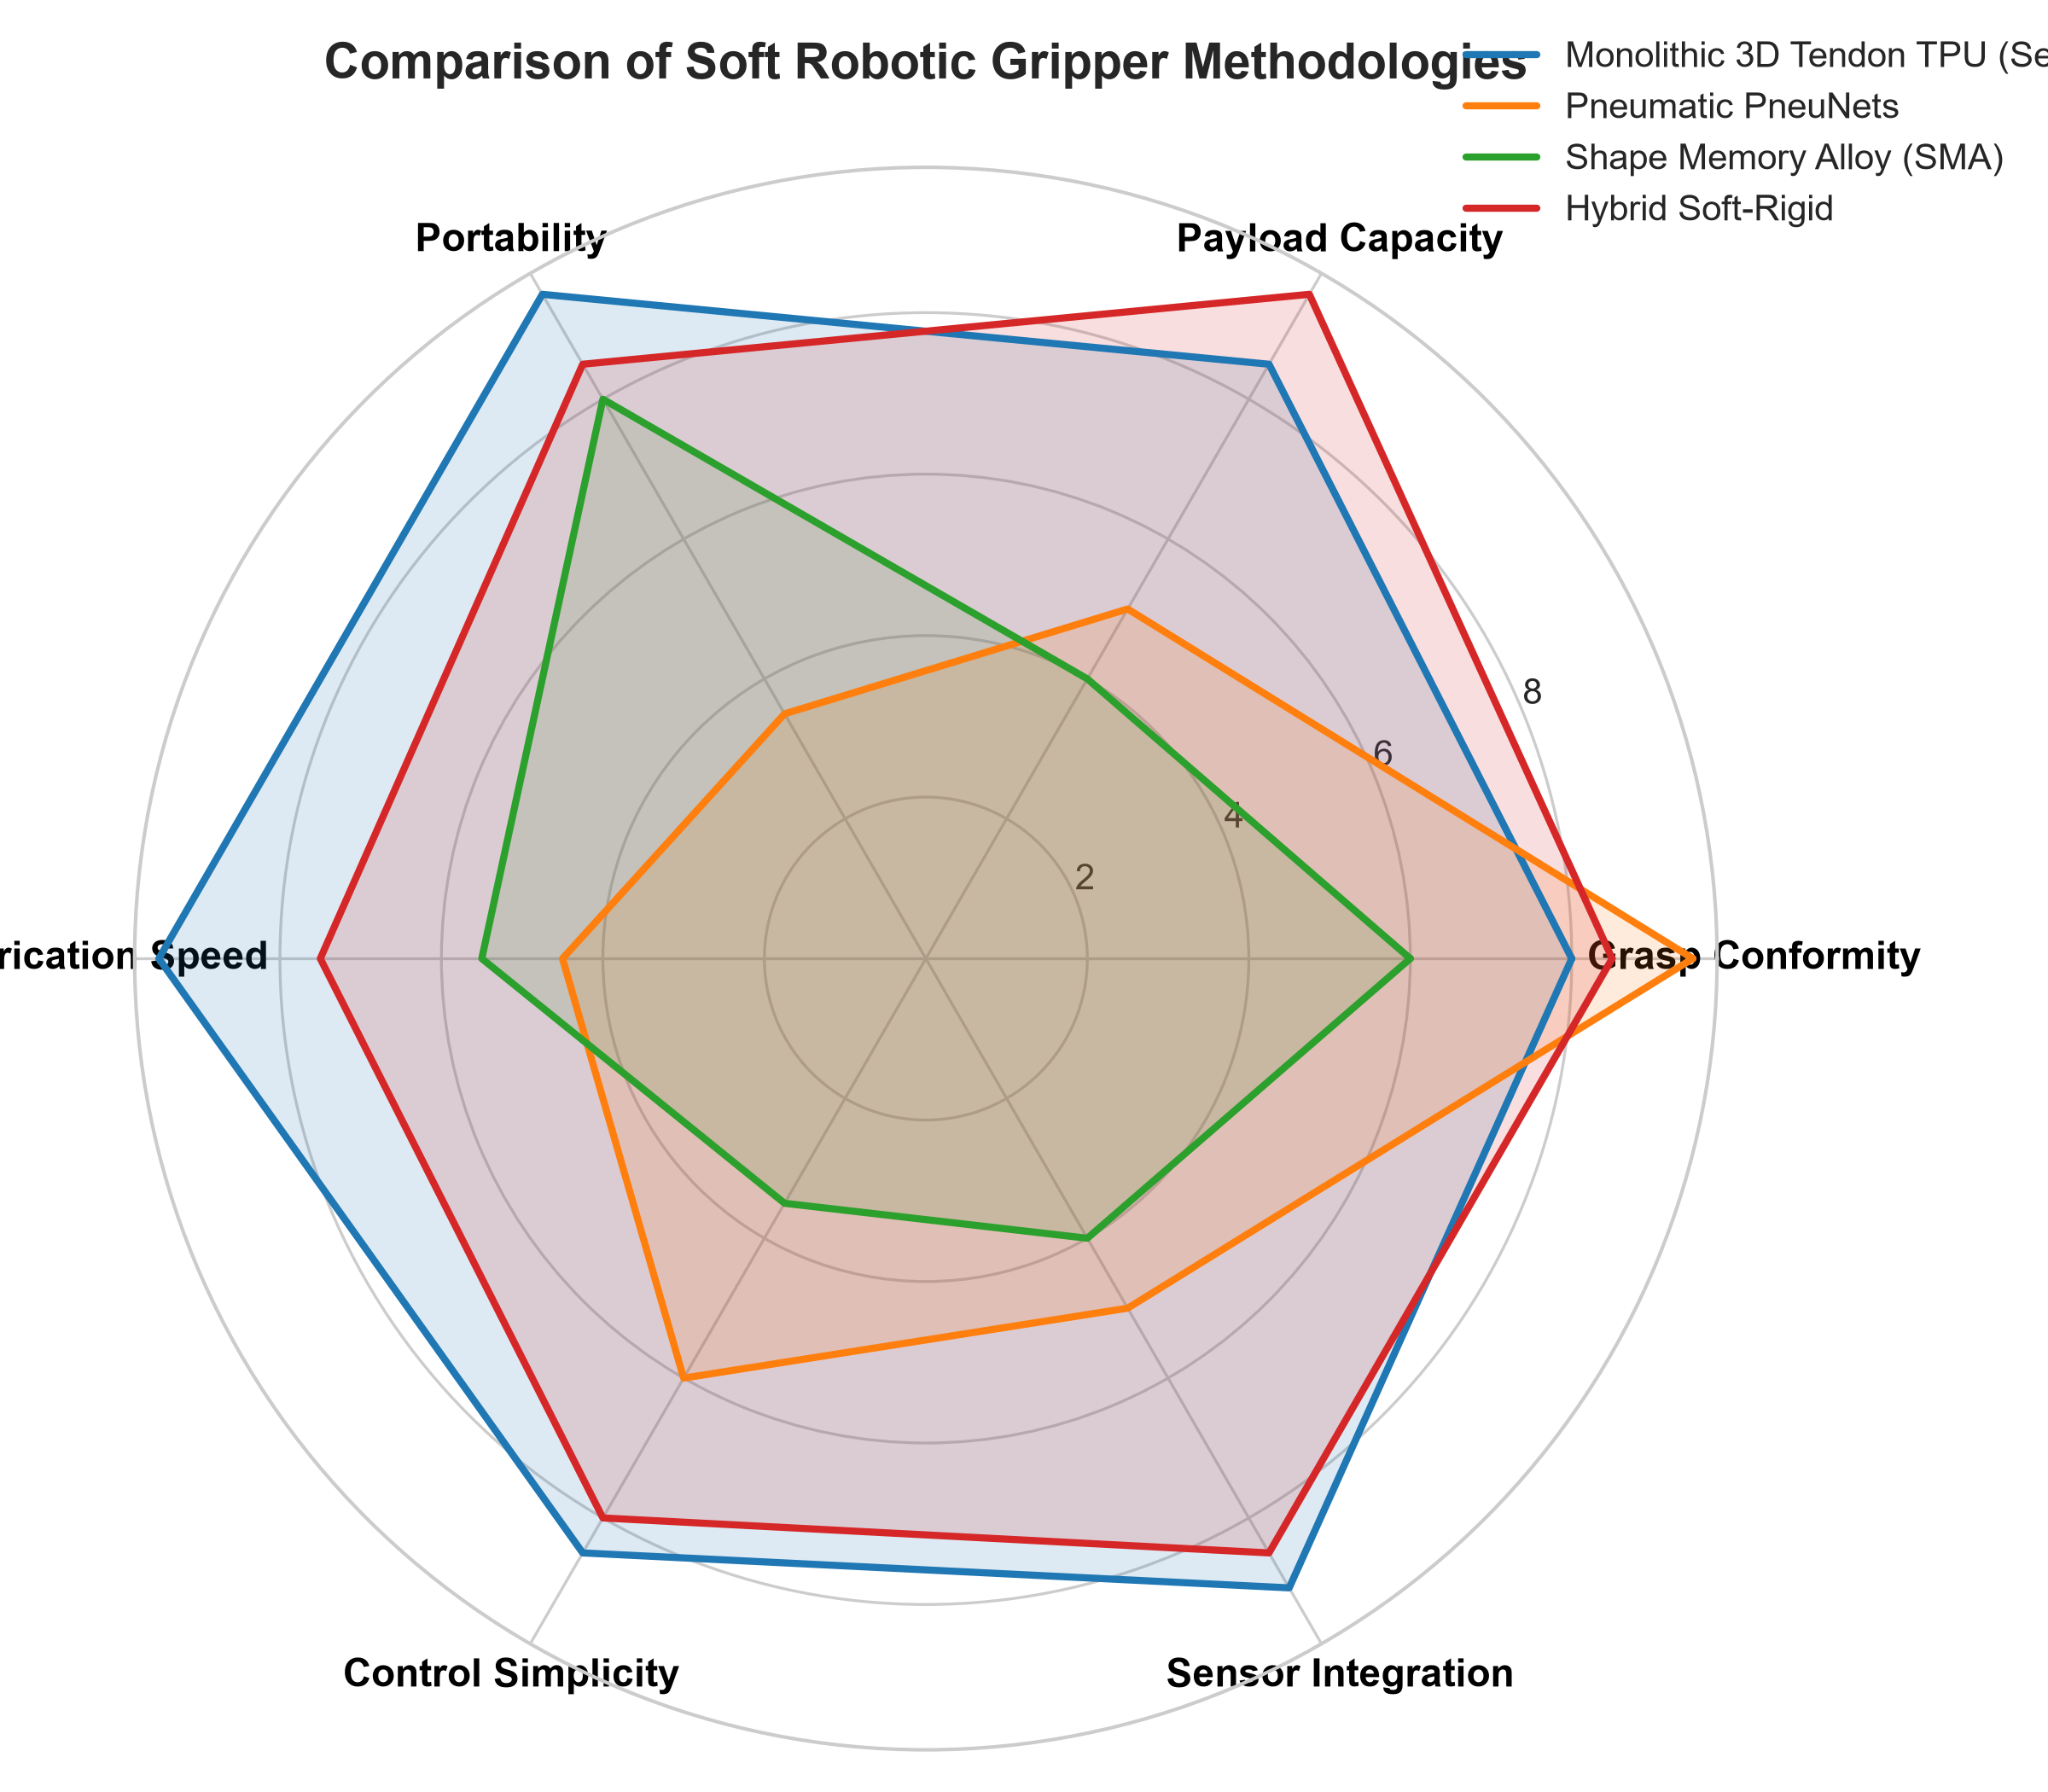
\includegraphics[width=0.75\textwidth]{../Figures and Diagrams/comparative_radar_chart.png}
    \caption{Multi-attribute radar comparison of candidate soft robotic gripper technologies.}
    \label{fig:radar_chart}
\end{figure}

\section{Identified Research Gaps}
A critical synthesis of the literature reveals five distinct research gaps that directly inform the technical direction of this BTP:
\begin{enumerate}
    \item \textbf{Research Gap 1: Structural Compliance vs. Payload Capacity Trade-off:} Soft pneumatic bladders buckle under lateral or torsional loads, limiting their capacity to lift payloads exceeding a few hundred grams. Compliant mechanisms that blend rigid finger phalanges with flexible living hinges can withstand substantial payload weights while maintaining contact compliance.
    \item \textbf{Research Gap 2: Sensor Delamination under Cyclic Bending:} Affixing planar thin-film sensors onto soft elastomers subjected to large tensile strain ($>50\%$) induces severe shear stresses at the adhesive interface, leading to peeling and catastrophic failure. There is a lack of geometric designs that isolate the sensing substrate from cyclic bending strain.
    \item \textbf{Research Gap 3: Absence of Compact Incipient Slip Detection:} Most slip-detecting robotic hands rely either on high-speed tactile cameras (e.g., GelSight) or complex multi-axis optical encoders. These approaches are computationally prohibitive, physically bulky, and cannot be integrated into lightweight, mobile soft grippers.
    \item \textbf{Research Gap 4: Neglect of Material Viscoelastic Hysteresis in Open-Loop Grasping:} Polymeric flexures exhibit time-dependent viscoelastic relaxation and strain history dependence. Traditional controllers ignore this, resulting in degraded positioning and force drift during sustained holds.
    \item \textbf{Research Gap 5: Disconnect Between Embedded Edge Control and High-Level Robotics Frameworks:} Prototype soft hands are frequently tethered to desktop PCs running MATLAB scripts. True industrial manipulation demands deterministic on-board microcontrollers (running real-time operating systems) integrated into modern distributed middleware (ROS 2).
\end{enumerate}

% ==================== CHAPTER 3 ====================
\chapter{Objectives and Scope of Work}

\section{Main Objective}
The central objective of this research project is to design, model, fabricate, and experimentally validate an integrated \textbf{Monolithic 3D-Printed Tendon-Driven Compliant Soft Robotic Gripper} featuring embedded piezoresistive tactile sensing and real-time edge processing on an ESP32 microcontroller, culminating in an autonomous closed-loop demonstration of incipient slip detection and force compensation.

\section{Specific Sub-Objectives}
To systematically achieve the primary objective across the two project phases (BTP-I and BTP-II), the following specific engineering sub-objectives are defined:
\begin{enumerate}
    \item \textbf{Mechanical & Kinematic Synthesis:} Synthesize a multi-finger compliant gripper architecture in SolidWorks, optimizing circular flexure living hinges to distribute bending stresses and incorporating low-friction radiused tendon channels alongside recessed sensor mounting beds.
    \item \textbf{Non-linear Computational FEA:} Formulate a hyperelastic constitutive model (Mooney-Rivlin / Yeoh) for TPU 95A in Ansys Mechanical, performing large-deflection structural simulations to verify that maximum Von Mises stresses remain safely below the material yield strength ($\sigma_{\text{max}} < \sigma_y$) and deriving the predictive tendon force vs. tip deflection relationship.
    \item \textbf{Additive Manufacturing Optimization:} Optimize direct-drive FDM 3D printing parameters (layer height, horizontal build orientation, $100\%$ concentric infill at hinge cores, extrusion temperature) to maximize inter-layer shear resistance and eliminate anisotropic delamination.
    \item \textbf{Analog Signal Conditioning & Acquisition:} Design and fabricate a custom analog interface circuit featuring an active op-amp buffer and a second-order Sallen-Key low-pass filter ($f_c = 20\text{ Hz}$) to eliminate high-frequency electromagnetic noise while extracting clean normal contact force data.
    \item \textbf{Real-Time FFT-Based Slip Detection:} Implement an on-chip Radix-4 256-point Fast Fourier Transform (FFT) algorithm running deterministically on ESP32 Core 0 at $1\text{ kHz}$ to detect high-frequency tactile micro-vibrations ($100 - 300\text{ Hz}$) indicative of incipient slip.
    \item \textbf{Deterministic Firmware & ROS 2 Integration:} Develop a dual-core FreeRTOS firmware pipeline executing closed-loop servomotor PWM torque modulation upon slip trigger within $<35\text{ ms}$, while publishing telemetry over micro-ROS to a host ROS 2 environment.
    \item \textbf{Experimental Benchmarking:} Quantify static gripping force, pull-out retention force, maximum payload-to-weight ratio, and slip-reaction latency across a standardized workpiece set (cylinders, spheres, fragile eggs, soft fruits).
\end{enumerate}

\section{Scope and Technical Boundaries}
\begin{itemize}
    \item \textbf{In-Scope:} Geometric parametric CAD modeling; non-linear hyperelastic structural FEA in Ansys; direct FDM 3D printing with TPU 95A and PLA; tactile sensor integration (FSR402); dual-core FreeRTOS firmware development; static force calibration and dynamic pull-out slip experimentation.
    \item \textbf{Out-of-Scope:} Industrial high-speed sorting ($>3\text{ m/s}$ linear accelerations); multi-axis shear force sensor arrays; underwater or vacuum grasping; explosive field testing.
\end{itemize}

% ==================== CHAPTER 4 ====================
\chapter{Proposed Methodology}

\section{Problem Description and System Architecture}
The proposed system addresses the challenge of grasping delicate, irregularly contoured workpieces without pre-existing dimensional models, while preventing accidental slippage during arm transport. 

Figure~\ref{fig:mechatronics} illustrates the unified mechatronic architecture connecting mechanical compliance, tactile sensing, edge processing, and actuation.

\begin{figure}[htbp]
    \centering
    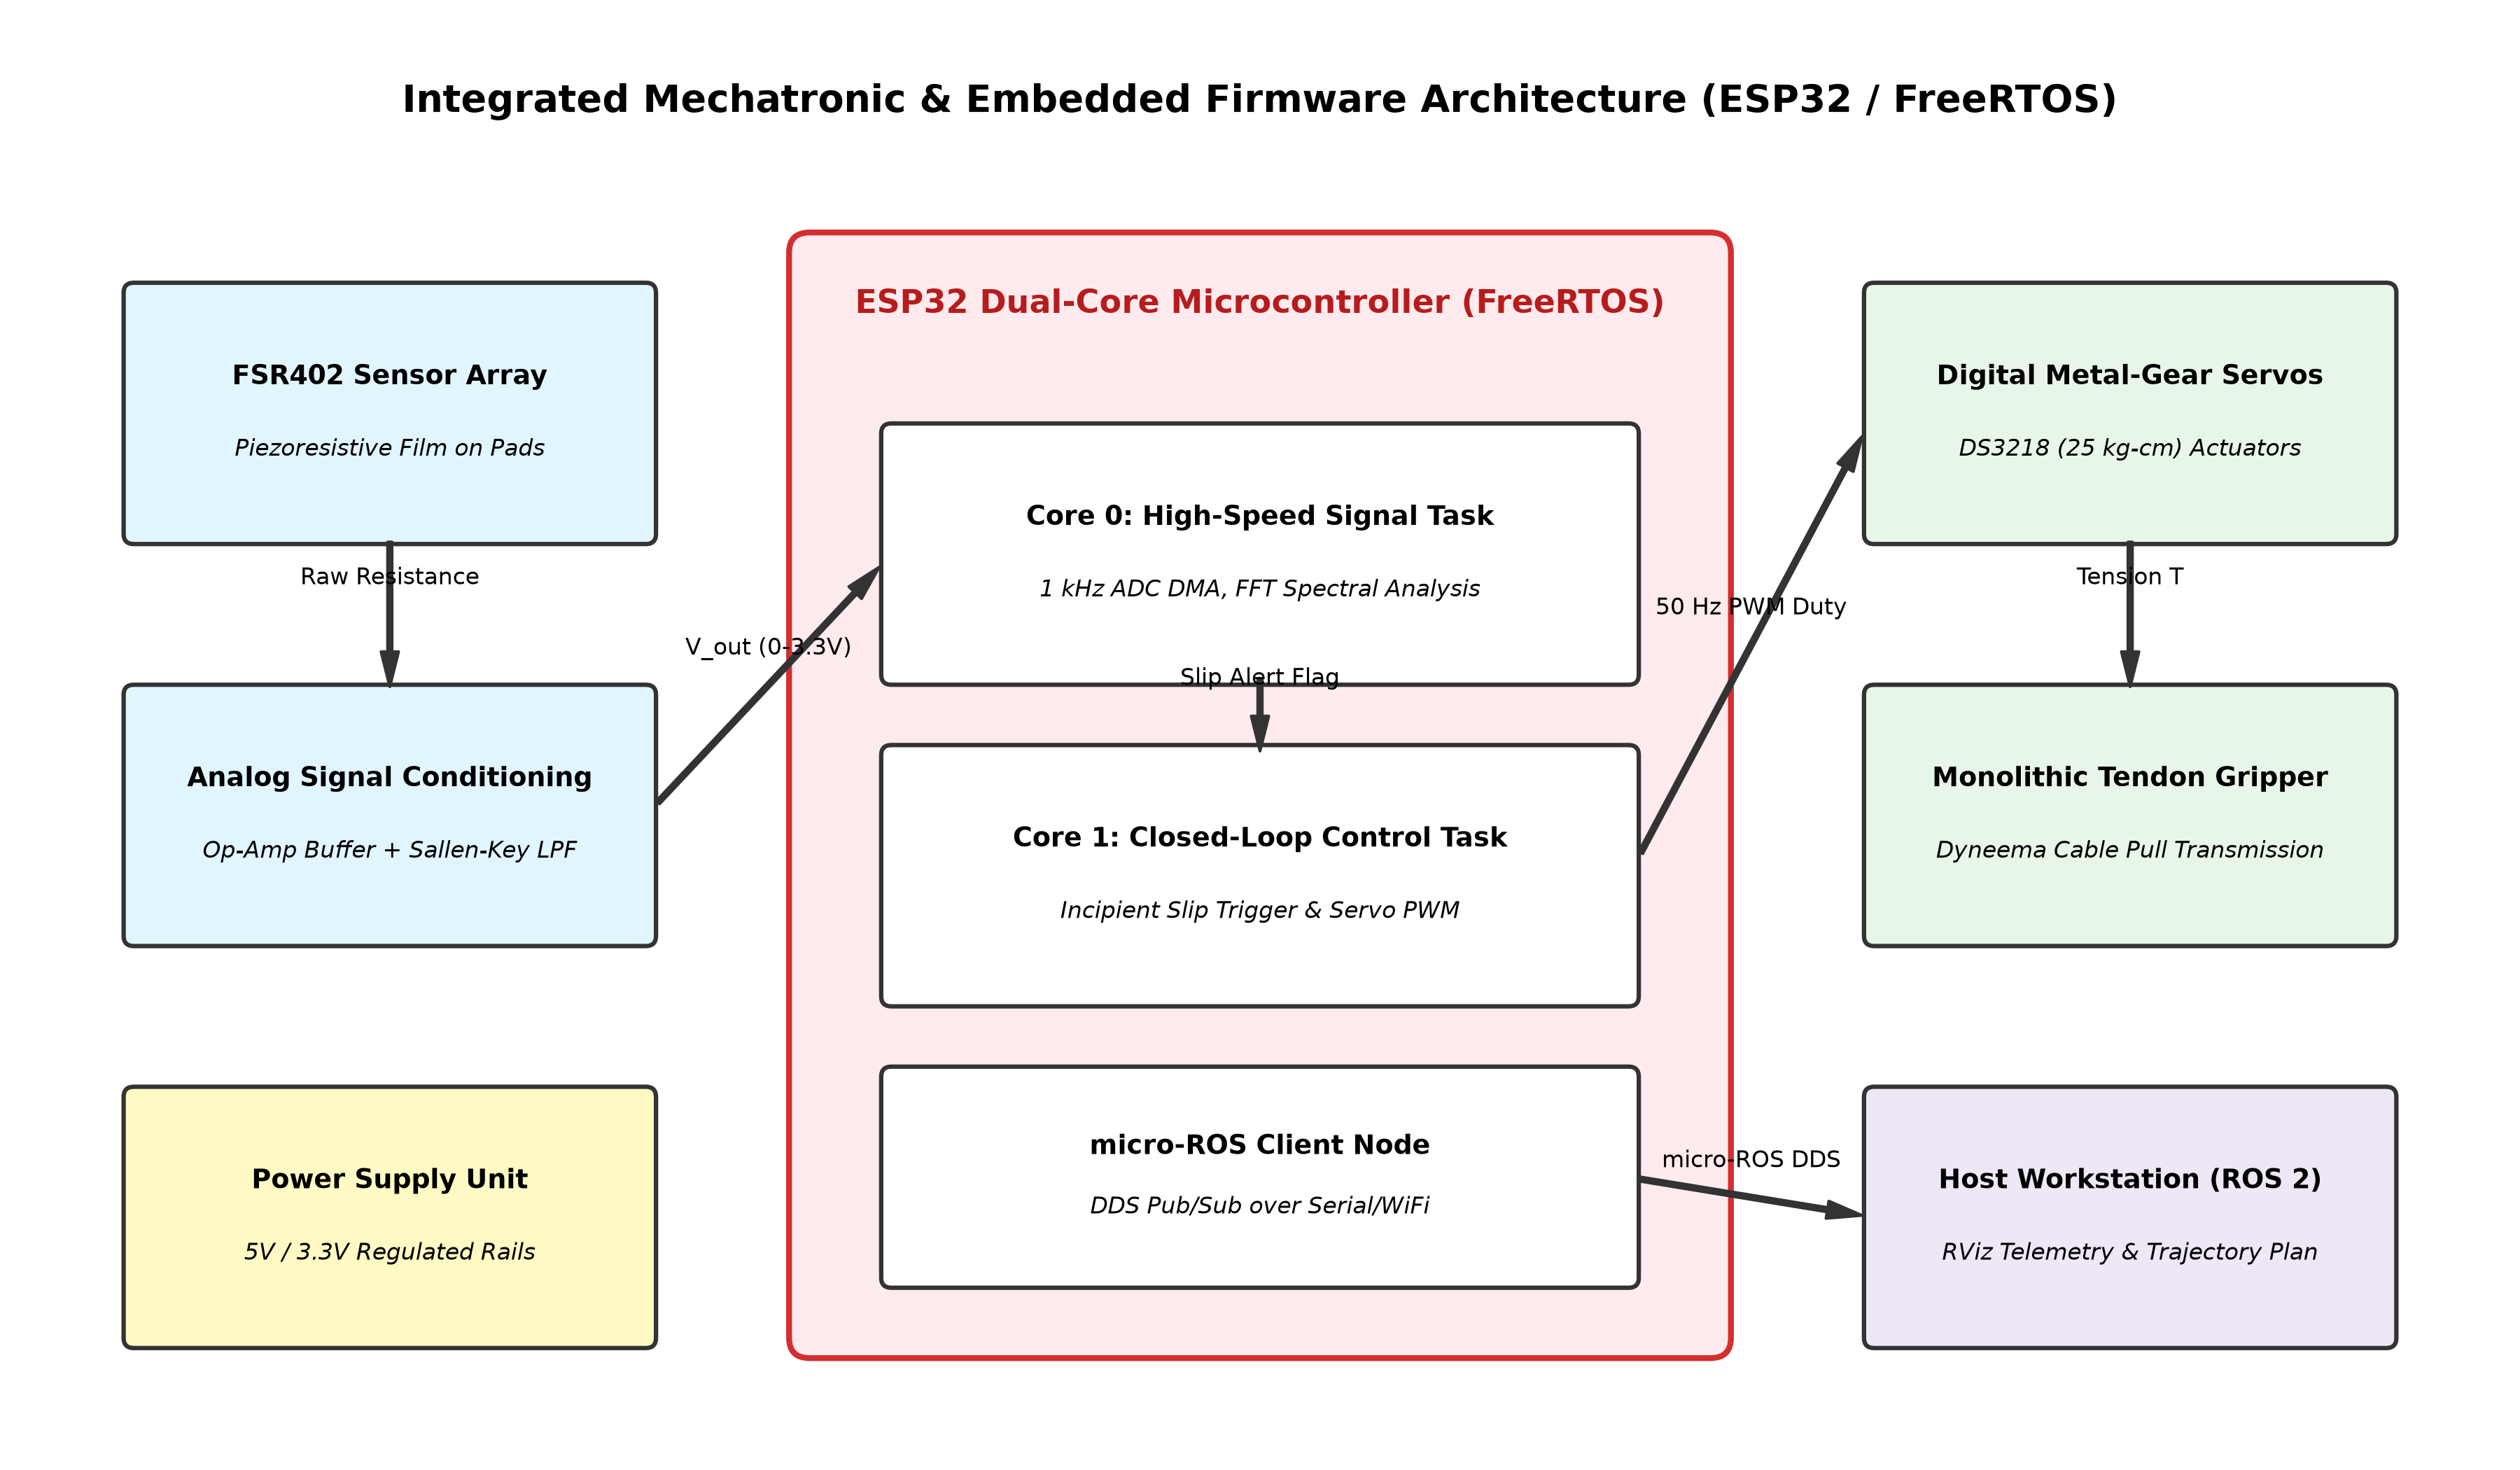
\includegraphics[width=0.95\textwidth]{../Figures and Diagrams/mechatronics_architecture.png}
    \caption{Integrated mechatronics and FreeRTOS embedded architecture for the compliant gripper.}
    \label{fig:mechatronics}
\end{figure}

\section{Kinematic Synthesis of the Monolithic Compliant Finger}
Unlike rigid linkages that require pins, bearings, and assembly fasteners, the proposed finger is a single continuous monolithic structure fabricated from flexible Thermoplastic Polyurethane (TPU 95A). Motion is governed by elastic deformation localized at three circular flexure living hinges replicating the metacarpophalangeal (MCP), proximal interphalangeal (PIP), and distal interphalangeal (DIP) joints of the human finger.

Figure~\ref{fig:kinematics} illustrates the kinematic topology, showing the unbent resting profile, the cable-driven bent profile, and the embedded sensor locations.

\begin{figure}[htbp]
    \centering
    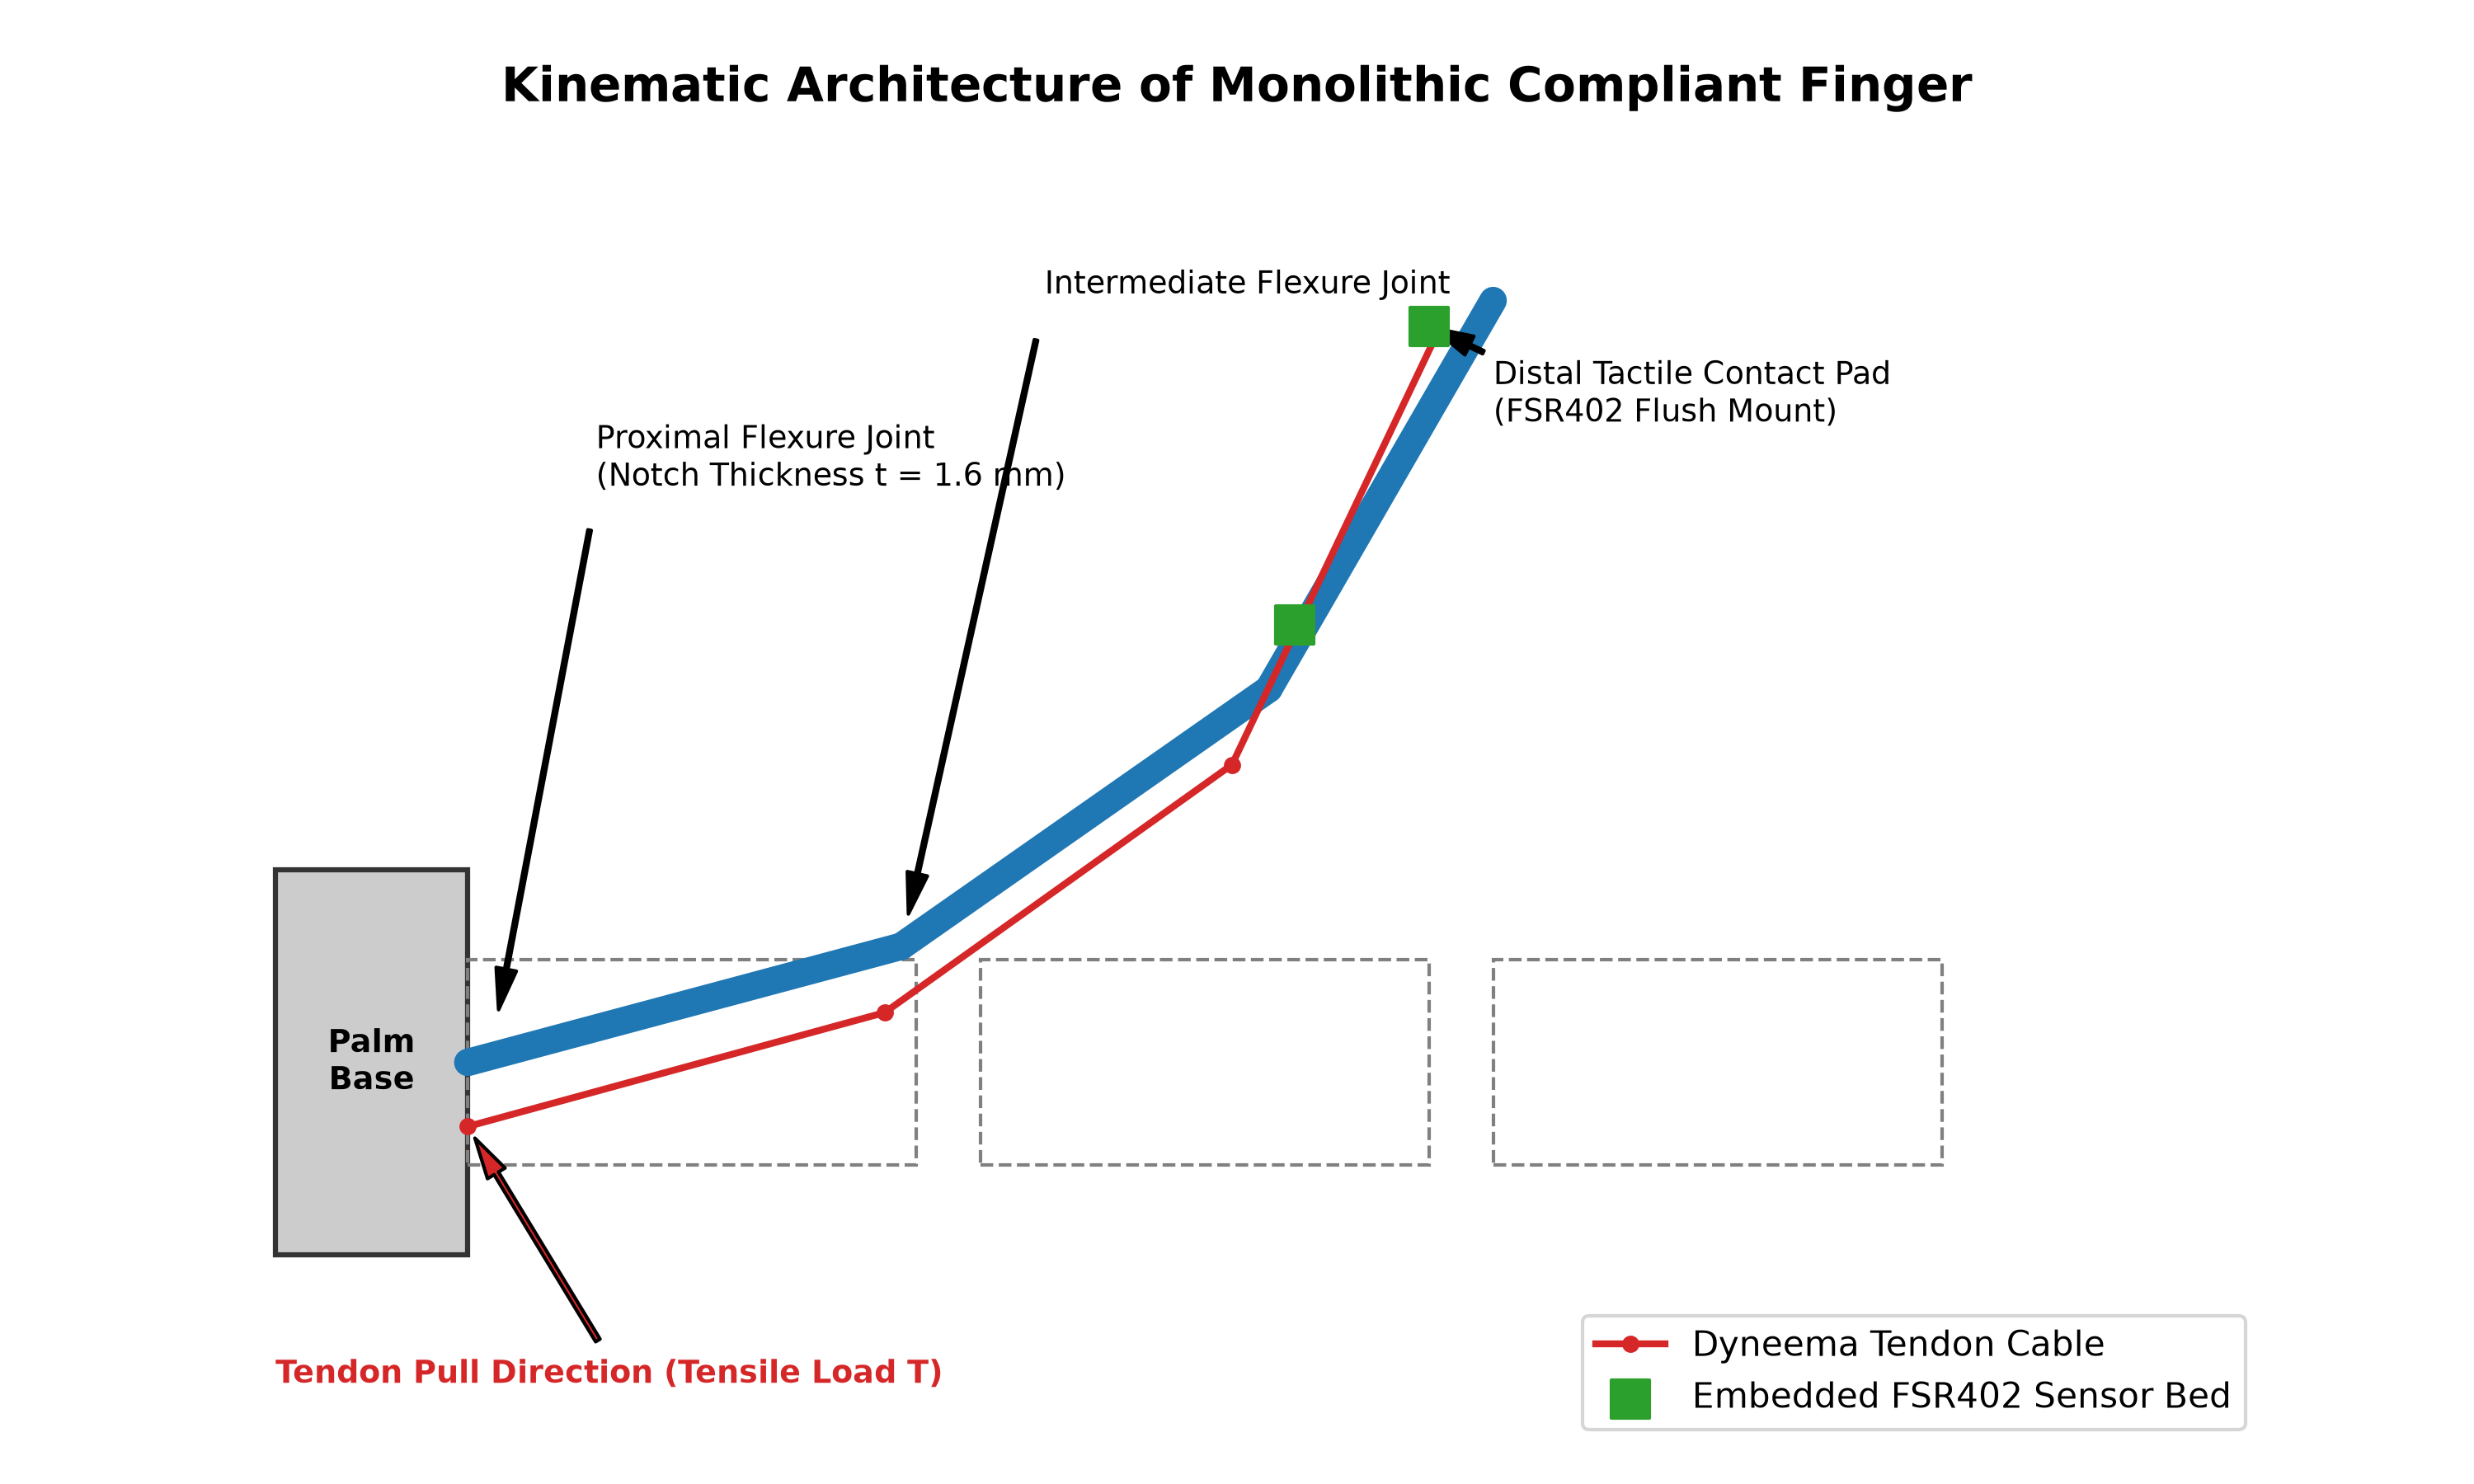
\includegraphics[width=0.9\textwidth]{../Figures and Diagrams/gripper_kinematics_diagram.png}
    \caption{Kinematic model of the monolithic compliant finger under tensile tendon loading.}
    \label{fig:kinematics}
\end{figure}

\subsection{Geometric Link Dimensions and Kinematic Topology}
The monolithic finger geometry adopts an anthropomorphic 3-phalanx kinematic configuration. The continuous flexible body is partitioned into three functional phalanx segments separated by localized circular living hinge flexures:
\begin{itemize}
    \item \textbf{Proximal Phalanx ($L_1 = 35.0\text{ mm}$):} Anchored directly to the rigid palm base flange; initiates primary angular deflection during early tendon stroke.
    \item \textbf{Intermediate Phalanx ($L_2 = 35.0\text{ mm}$):} Medial link segment that conforms around the lateral flanks of grasped objects.
    \item \textbf{Distal Phalanx ($L_3 = 35.0\text{ mm}$):} Fingertip segment incorporating an integrated $5.0\text{ mm}$ radiused contact pad and a precision circular recessed pocket ($\phi = 18.3\text{ mm}$, depth $0.6\text{ mm}$) configured to seat the Interlink FSR402 thin-film sensor flush with the gripping face.
\end{itemize}
With circular notch gaps of $g_1 = g_2 = 5.0\text{ mm}$ and the distal fingertip extension, the total unbent finger length is $L_{\text{total}} = 115.0\text{ mm}$. The beam cross-section features a width of $w = 20.0\text{ mm}$ and height of $h = 16.0\text{ mm}$, providing substantial lateral torsional stiffness to prevent out-of-plane twisting while permitting low-resistance in-plane flexing. Symmetrically arranged on an $80.0\text{ mm}$ pitch circle diameter (PCD) palm base, the fingers deliver a combined envelope grasping range from $\phi = 25.0\text{ mm}$ to $\phi = 85.0\text{ mm}$. Table~\ref{tab:link_dimensions} details the complete geometric and kinematic design specifications.

\begin{table}[htbp]
\centering
\small
\caption{Geometric link lengths and kinematic dimensions of the monolithic compliant finger.}
\label{tab:link_dimensions}
\begin{tabularx}{\textwidth}{l p{3.2cm} c X}
\toprule
\textbf{Parameter} & \textbf{Symbol} & \textbf{Value} & \textbf{Functional / Kinematic Rationale} \\
\midrule
Proximal Phalanx Length & $L_1$ & $35.0\text{ mm}$ & Matches human proximal phalanx; provides primary envelope wrap. \\
Intermediate Phalanx Length & $L_2$ & $35.0\text{ mm}$ & Replicates intermediate phalanx; guides medial curvature. \\
Distal Phalanx Length & $L_3$ & $35.0\text{ mm}$ & Fingertip segment; houses recessed FSR402 contact pad ($+5\text{ mm}$ tip). \\
Total Finger Beam Length & $L_{\text{total}}$ & $115.0\text{ mm}$ & Total effective finger length ($L_1 + g_1 + L_2 + g_2 + L_3 + \text{tip}$). \\
Finger Cross-Section Width & $w$ & $20.0\text{ mm}$ & Ensures lateral torsional rigidity and stable planar bending. \\
Finger Cross-Section Height & $h$ & $16.0\text{ mm}$ & Accommodates internal $2\text{ mm}$ tendon conduit with $7\text{ mm}$ wall clearance. \\
Flexure Throat Thickness & $t$ & $1.6\text{ mm}$ & Optimized for low bending resistance while maintaining structural integrity. \\
Circular Notch Radius & $r$ & $2.5\text{ mm}$ & Distributes bending stresses to minimize localized stress concentration. \\
Notch Opening Gap & $g$ & $5.0\text{ mm}$ & Provides clear angular clearance for up to $30^\circ$ deflection per hinge. \\
Tendon Moment Arm Offset & $r_{\text{cable}}$ & $6.0\text{ mm}$ & Distance from flexure neutral axis to tendon channel centerline. \\
Tendon Conduit Diameter & $\phi_c$ & $2.0\text{ mm}$ & Lined with low-friction micro-PTFE sleeve (OD $2.0\text{ mm}$, ID $1.0\text{ mm}$). \\
Distal Sensor Recess & $\phi_{\text{sensor}} \times d$ & $\phi 18.3 \times 0.6\text{ mm}$ & Flush mounting bed for Interlink FSR402 active sensing area. \\
Base Pitch Circle Diameter & $\phi_{\text{base}}$ & $80.0\text{ mm}$ & Symmetrical 3-finger equilateral radial mounting flange. \\
Target Grasp Diameter & $\phi_{\text{grasp}}$ & $25.0 - 85.0\text{ mm}$ & Adaptive envelope grasping range for domestic and industrial items. \\
Maximum Tip Curl Angle & $\theta_{\text{total}}$ & $\approx 82^\circ$ & Cumulative angular deflection under $12 - 15\text{ mm}$ tendon stroke. \\
\bottomrule
\end{tabularx}
\end{table}

\subsection{Mechanical Design Constraints and Payload Specifications}
To ensure structural durability, non-destructive fatigue life, and robust grasping performance across diverse workpiece geometries, the compliant gripper is governed by well-defined mechanical, manufacturing, and operational constraints:
\begin{itemize}
    \item \textbf{Structural Stress and Elastic Strain Constraints:} Under maximum tendon tension, bending stress concentrates at the throat of the circular flexure living hinges. The maximum allowable localized Von Mises stress is restricted to $\sigma_{\text{max}} \le 22.0\text{ MPa}$. With the tensile yield strength of 3D-printed TPU 95A established at $\sigma_y \approx 48 - 52\text{ MPa}$, this ensures a structural safety factor of $SF = \sigma_y / \sigma_{\text{max}} \ge 2.2$. This margin guarantees that all hinge deformations remain purely within the linear-elastic recovery regime, preventing permanent set, plastic necking, and low-cycle fatigue failure over $>100,000$ cycles. The maximum outer-fiber tensile strain is constrained to $\varepsilon_{\text{max}} \le 45\%$, well below the material's ultimate failure strain ($>450\%$).
    \item \textbf{Additive Manufacturing Constraints:} To avoid anisotropic delamination, all fingers are constrained to be 3D printed flat in the horizontal X-Y build plane. This guarantees that tensile bending stresses along the living hinge throat align parallel with continuous, uninterrupted extruded polymer road contours rather than across inter-layer Z-boundaries. Infill at the hinge throats is specified as $100\%$ concentric.
    \item \textbf{Actuation and Transmission Constraints:} Actuation is achieved via single-acting high-strength Dyneema braided cable (breaking strength $>250\text{ N}$). Return extension is fully passive, powered by the stored elastic strain energy of the deformed living hinges ($E_{\text{strain}} = \sum \frac{1}{2} K_{\theta, i} \theta_i^2$). To mitigate friction losses along the internal routing conduits, the channel is lined with micro-PTFE tubing ($\mu_f \le 0.08$), ensuring that nominal tendon pull remains $T_{\text{nom}} \approx 12.5\text{ N}$ with a peak operating ceiling of $T_{\text{max}} \le 25.0\text{ N}$.
    \item \textbf{Payload Capacity and Dynamic Grasp Specifications:} The gripper is engineered to handle a rated dynamic payload of $800 - 1500\text{ g}$ ($0.8 - 1.5\text{ kg}$) across cylinders, spheres, and rectangular objects, with a peak static envelope holding capacity of up to $2.0\text{ kg}$ ($2000\text{ g}$). With a total estimated gripper self-mass under $450\text{ g}$ (including 3 TPU fingers, PLA palm, servo mounting brackets, and spools), the design achieves an exceptional payload-to-weight ratio exceeding $3:1$ (and up to $4.4:1$ in static lock), outperforming conventional fluidic elastomer grippers ($<1.5:1$). Controlled normal clamping force spans $0.1\text{ N}$ (for delicate workpieces such as raw eggs and ripe fruit) to $20.0\text{ N}$ (for robust industrial parts), coupled with a dynamic slip-reflex latency under $35\text{ ms}$.
\end{itemize}

\begin{table}[htbp]
\centering
\small
\caption{Summary of mechanical design constraints, actuation limits, and payload specifications.}
\label{tab:design_constraints}
\begin{tabularx}{\textwidth}{l l c X}
\toprule
\textbf{Domain} & \textbf{Design Parameter} & \textbf{Target / Limit} & \textbf{Governing Constraint and Engineering Rationale} \\
\midrule
\multirow{3}{*}{\textbf{Structural / Stress}} 
& Peak Von Mises Stress & $\sigma_{\text{max}} \le 22.0\text{ MPa}$ & Safe margin below TPU 95A yield strength ($\sigma_y \approx 50\text{ MPa}$). \\
& Safety Factor (Yield) & $SF \ge 2.2$ & Prevents permanent plastic deformation and low-cycle fatigue. \\
& Maximum Bending Strain & $\varepsilon_{\text{max}} \le 45\%$ & Remains within reversible elastic regime (TPU elongation $>450\%$). \\
\midrule
\multirow{2}{*}{\textbf{Manufacturing}} 
& Build Orientation & Flat in X-Y Plane & Ensures tensile bending stresses align with continuous filament beads. \\
& Infill Density at Hinges & $100\%$ Concentric & Eliminates internal voids and prevents inter-layer delamination. \\
\midrule
\multirow{3}{*}{\textbf{Transmission}} 
& Tendon Tensile Force & $T_{\text{nom}} = 12.5\text{ N}$ ($T_{\text{max}} \le 25\text{ N}$) & Safe operating load for high-torque digital servomotor (MG996R). \\
& Tendon Stroke & $\Delta x = 12 - 15\text{ mm}$ & Delivers $82^\circ$ full envelope wrap across 3 living hinges. \\
& Conduit Friction Coeff. & $\mu_f \le 0.08$ & Micro-PTFE sleeve minimizes Capstan tension loss along curved path. \\
\midrule
\multirow{6}{*}{\textbf{Payload \& Force}} 
& Rated Grasp Payload & $800 - 1500\text{ g}$ ($0.8 - 1.5\text{ kg}$) & Operational capacity across irregular cylinders, spheres, and boxes. \\
& Peak Static Payload & Up to $2.0\text{ kg}$ ($2000\text{ g}$) & Form-closure envelope grasp holding capacity under full lock. \\
& Gripper Self-Weight & $< 450\text{ g}$ & Total mass of 3 fingers, palm base, servo mount, and spools. \\
& Payload-to-Weight Ratio & $> 3:1$ (up to $4.4:1$) & Exceeds conventional fluidic/pneumatic soft grippers ($< 1.5:1$). \\
& Normal Clamping Force & $0.1 - 20.0\text{ N}$ & Controllable range from fragile eggs ($0.5\text{ N}$) to rigid objects. \\
& Closed-Loop Latency & $< 35\text{ ms}$ & Dynamic FFT reflex to servomotor torque tightening on slip. \\
\bottomrule
\end{tabularx}
\end{table}



\subsection{Pseudo-Rigid-Body Modeling (PRBM)}
To analyze the large deflections of the living hinges, the Pseudo-Rigid-Body Model (PRBM) developed by Howell \cite{howell2001compliant} is applied. A circular flexure notch of thickness $t$, radius $r$, and width $w$ subjected to an applied bending moment $M$ is modeled as a rigid link rotating about a characteristic pivot with equivalent torsional spring stiffness $K_\theta$:
\begin{equation}
    K_\theta = \frac{E \cdot w \cdot t^{2.5}}{9 \pi \sqrt{r}}
\end{equation}
where $E$ is the instantaneous flexural modulus of the TPU material. Under a tensile cable load $T$ acting at a moment arm distance $r_{\text{cable}}$ from the neutral axis, the angular deflection $\theta_i$ of each flexure joint satisfies moment equilibrium:
\begin{equation}
    T \cdot r_{\text{cable}} = K_{\theta, i} \cdot \theta_i + M_{\text{contact}}
\end{equation}

\subsection{Tendon Friction and Capstan Effect}
The Dyneema cable is routed through internal curved guides within the finger body. The transmission of tensile force from the base servo to the distal tip is governed by the Capstan formulation:
\begin{equation}
    T_{\text{distal}} = T_{\text{base}} \cdot \exp\left(-\sum_{i=1}^3 \mu_f \theta_i\right)
\end{equation}
where $\mu_f$ is the Coulomb coefficient of friction between the braided Dyneema tendon and the 3D-printed internal conduit (minimized to $\mu_f \approx 0.08$ via low-friction micro-PTFE sleeve inserts).


\section{Grasping Mechanics, Contact Sequence, and Target Workpieces}

\subsection{Underactuated Mechanical Intelligence and Multi-Phase Contact Sequence}
Unlike conventional rigid industrial grippers that demand multi-axis servomotor coordination and complex inverse kinematic trajectory planning for every unique workpiece contour, the proposed soft robotic finger utilizes \textit{underactuated mechanical intelligence}. A single tensile tendon actuates three independent revolute degrees of freedom (MCP, PIP, and DIP living hinges). The grasping progression evolves across five discrete mechanical phases:
\begin{enumerate}
    \item \textbf{Phase 0 (Equilibrium Rest Configuration):} The Dyneema tendon is slack ($T = 0\text{ N}$). All three living hinges remain unbent in their straight manufactured posture ($\theta_1 = \theta_2 = \theta_3 = 0^\circ$), establishing an open grasp envelope ($\phi \approx 90 - 110\text{ mm}$).
    \item \textbf{Phase 1 (Free In-Flight Flexure):} The base servomotor rotates the drive spool, generating cable tension $T$. This applies an inward bending moment $M = T \cdot r_{\text{cable}}$ across all three flexure notches simultaneously via the $6.0\text{ mm}$ neutral-axis offset. All phalanges flex inward proportionally to their torsional compliance ($K_{\theta, i}$).
    \item \textbf{Phase 2 (Proximal Contact and Kinematic Motion Arrest):} As the finger sweeps inward, the proximal phalanx ($L_1$) or intermediate phalanx ($L_2$) impinges upon the exterior surface of the workpiece. The normal contact reaction force creates an opposing moment $M_{\text{contact}} = F_n \cdot d_{\text{contact}}$ that balances the tendon moment at the proximal hinge ($K_{\theta, 1}\theta_1 + M_{\text{contact}} = T \cdot r_{\text{cable}}$), arresting further angular deflection of the proximal link.
    \item \textbf{Phase 3 (Continuous Routing and Distal Adaptive Curling):} Because the braided Dyneema tendon slides freely through low-friction micro-PTFE sleeve liners ($\mu_f \le 0.08$), the continuing spool rotation channels the remaining tensile force downstream past the arrested proximal phalanx into the unrestrained intermediate and distal living hinges ($K_{\theta, 2}$, $K_{\theta, 3}$). The intermediate and distal phalanges curl automatically around the irregular contour of the object until multi-point contact equilibrium is established. This passive morphological conformity occurs purely through elastic structural compliance, requiring zero sensory feedback or algorithmic path planning.
    \item \textbf{Phase 4 (Stable Grasp Lock and Tactile Sensor Activation):} The distal phalangeal contact pad presses flush against the workpiece surface, transmitting contact normal force directly into the embedded Interlink FSR402 thin-film sensor. As the calibrated normal force achieves the target setpoint ($0.5 - 20.0\text{ N}$), the FreeRTOS motor control task transitions the servomotor into static holding torque mode.
    \item \textbf{Phase 5 (Passive Strain-Energy Elastic Release):} When release is commanded, the servomotor unwinds the tendon spool. The elastic strain energy stored in the deformed TPU living hinges ($E_{\text{strain}} = \sum_{i=1}^3 \frac{1}{2} K_{\theta, i} \theta_i^2$) acts as an internal distributed restoring spring, instantly popping the fingers back to their straight resting posture without requiring reverse pushrods or dual-acting actuation.
\end{enumerate}

\subsection{Grasping Modalities: Power Envelope Grasp versus Precision Pinch Grasp}
The kinematic architecture of the 3-finger gripper supports two primary grasping modalities depending on target workpiece dimensions and fragility:
\begin{itemize}
    \item \textbf{Power Envelope Grasp (Form Closure):} Suited for medium-to-large objects ($\phi = 25 - 85\text{ mm}$, mass up to $1.5 - 2.0\text{ kg}$). The three phalanges completely wrap around the workpiece boundary, maximizing contact surface area. High geometric form-closure and distributed frictional engagement lock the object securely against external dynamic accelerations during manipulator transport.
    \item \textbf{Precision Fingertip Pinch Grasp (Force Closure):} Suited for small, thin, or delicate workpieces ($\phi = 5 - 25\text{ mm}$, e.g., thin electronic components, test tube necks, pens, and coins). Only the distal phalangeal contact pads ($L_3$) press against opposing sides of the workpiece. The high static friction coefficient of 3D-printed TPU ($\mu_s \approx 0.6 - 0.8$) provides non-slip stability under low normal clamping forces ($0.1 - 2.0\text{ N}$), preventing structural damage to brittle workpieces.
\end{itemize}

\subsection{Bio-Inspired Anthropomorphic Equivalence and the Human Tactile Reflex Arc}
The design of the compliant gripper embodies direct bio-inspired structural and functional parallels to the human hand:
\begin{itemize}
    \item \textbf{Kinematic Skeletal Equivalence:} Replicates the three-phalanx kinematic chain of the human index finger (Proximal, Middle, and Distal Phalanges) and three rotational joints (Metacarpophalangeal [MCP], Proximal Interphalangeal [PIP], and Distal Interphalangeal [DIP]), replacing mechanical pins and bearings with monolithic circular flexure living hinges.
    \item \textbf{Flexor Tendon Sheath Biomechanics:} Emulates the human deep flexor tendon (\textit{flexor digitorum profundus}) running through its synovial flexor sheath (\textit{vagina fibrosa digitorum}) by routing high-tensile Dyneema cable through low-friction micro-PTFE conduits embedded within the finger core.
    \item \textbf{Cutaneous Mechanoreceptor Reflex Arc (Meissner's Corpuscles):} In human glabrous skin, Fast-Adapting Type I (FA-I / Meissner) mechanoreceptors do not measure static clamping pressure; instead, they fire rapid bursts of action potentials in response to high-frequency shear micro-vibrations ($100 - 300\text{ Hz}$) generated during the microscopic slip of papillary epidermal ridges across the object surface. This sensory volley triggers an involuntary spinal reflex arc that boosts grip force within $30 - 40\text{ ms}$ before macro-slip occurs. The proposed mechatronic system mirrors this biological reflex: the FSR402 sensor detects high-frequency tactile micro-vibrations, the ESP32 performs on-chip 256-point Radix-4 FFT spectral analysis in the $100 - 300\text{ Hz}$ band on Core 0, and triggers a sub-35 ms servomotor torque compensation interrupt on Core 1.
\end{itemize}

\subsection{Target Workpiece Library and Physical Compatibility Matrix}
To evaluate gripper versatility across unstructured environments, a standardized workpiece library is established spanning agriculture, biomedical handling, domestic food packaging, and industrial assembly. Table~\ref{tab:workpiece_library} details the dimensional envelope, mass range, grasping modality, and operational force requirements for each target class.

\begin{table}[htbp]
\centering
\small
\caption{Target workpiece library, dimensional envelope, and grasping compatibility matrix.}
\label{tab:workpiece_library}
\begin{tabularx}{\textwidth}{l p{2.6cm} c c c c X}
\toprule
\textbf{Application Domain} & \textbf{Target Workpiece} & \textbf{Envelope ($\phi$ / Dim.)} & \textbf{Mass Range} & \textbf{Grasp Mode} & \textbf{Clamping Force} & \textbf{Handling Challenge \& Soft Compliance Benefit} \\
\midrule
\multirow{2}{*}{\textbf{Agriculture}} 
& Ripe Tomato / Peach & $\phi 50 - 75\text{ mm}$ & $120 - 250\text{ g}$ & Envelope & $0.8 - 2.0\text{ N}$ & Thin skin bruises easily; compliant living hinges distribute contact pressure safely. \\
& Fresh Strawberry & $\phi 25 - 40\text{ mm}$ & $20 - 50\text{ g}$ & Pinch & $0.3 - 0.8\text{ N}$ & Highly delicate surface; fingertip compliance and low force threshold prevent bruising. \\
\midrule
\multirow{2}{*}{\textbf{Biomedical}} 
& Glass Vaccine Vial & $\phi 22 - 32\text{ mm}$ & $35 - 80\text{ g}$ & Envelope & $1.5 - 3.5\text{ N}$ & Smooth low-friction glass; high TPU static friction ($\mu_s \approx 0.7$) prevents slipping. \\
& Thin Glass Test Tube & $\phi 15 - 25\text{ mm}$ & $25 - 60\text{ g}$ & Pinch & $0.8 - 2.0\text{ N}$ & Brittle cylindrical glass; pinch grasp avoids radial crushing stress concentrations. \\
\midrule
\multirow{2}{*}{\textbf{Food \& Domestic}} 
& Raw Chicken Egg & $\phi 42 - 58\text{ mm}$ & $55 - 70\text{ g}$ & Envelope & $0.5 - 1.5\text{ N}$ & Brittle calcareous shell; multi-point conformal wrap prevents point-load shell fracture. \\
& Electric Light Bulb & $\phi 60 - 80\text{ mm}$ & $40 - 75\text{ g}$ & Envelope & $0.8 - 2.0\text{ N}$ & Fragile spherical glass envelope; conformal wrap grasps contoured globe reliably. \\
\midrule
\multirow{2}{*}{\textbf{Industrial}} 
& Aluminum Cylinder & $\phi 40 - 70\text{ mm}$ & $400 - 1200\text{ g}$ & Envelope & $8.0 - 18.0\text{ N}$ & Heavy rigid metallic part; high-torque envelope lock securely supports up to $1.5\text{ kg}$ payload. \\
& Prismatic Carton Box & $50 \times 60 \times 90\text{ mm}$ & $250 - 800\text{ g}$ & Envelope & $4.0 - 10.0\text{ N}$ & Flat geometric boundaries; compliant living hinges adapt passively to angular corners. \\
\bottomrule
\end{tabularx}
\end{table}

\section{Non-linear Hyperelastic Constitutive Modeling for FEA}
Standard linear elasticity cannot capture the non-linear, strain-stiffening behavior of TPU 95A under large flexural deformation. Therefore, the material is modeled as an isotropic, nearly-incompressible hyperelastic continuum. The strain energy density function $W$ is formulated using the 2-Parameter Mooney-Rivlin model \cite{mooney1940theory}:
\begin{equation}
    W = C_{10}(I_1 - 3) + C_{01}(I_2 - 3) + \frac{1}{D_1}(J - 1)^2
\end{equation}
where $I_1$ and $I_2$ are the first and second deviatoric strain invariants defined in terms of principal stretch ratios $\lambda_i$:
\begin{equation}
    I_1 = \lambda_1^2 + \lambda_2^2 + \lambda_3^2, \quad I_2 = \lambda_1^2 \lambda_2^2 + \lambda_2^2 \lambda_3^2 + \lambda_3^2 \lambda_1^2
\end{equation}
$J = \det(\mathbf{F}) = \lambda_1 \lambda_2 \lambda_3 \approx 1$ represents volumetric change, $C_{10}$ and $C_{01}$ are empirical material constants determined from uniaxial tensile testing of TPU 95A ($C_{10} \approx 2.45\text{ MPa}$, $C_{01} \approx 1.15\text{ MPa}$), and $D_1$ is the incompressibility parameter.

In Ansys Mechanical, the 3D geometry is discretized using higher-order 20-node hexahedral elements (SOLID186) with quadratic displacement shape functions to eliminate shear locking. A non-linear Newton-Raphson solver with automatic time stepping evaluates geometric non-linearities (Large Deflection `ON') to compute the stress tensor $\mathbf{\sigma}$:
\begin{equation}
    \mathbf{\sigma} = \frac{2}{J} \left[ \left(\frac{\partial W}{\partial I_1} + I_1 \frac{\partial W}{\partial I_2}\right) \mathbf{B} - \frac{\partial W}{\partial I_2} \mathbf{B}^2 \right] + p \mathbf{I}
\end{equation}
where $\mathbf{B} = \mathbf{F} \mathbf{F}^T$ is the left Cauchy-Green deformation tensor and $p$ is the hydrostatic pressure Lagrange multiplier.

\section{Tactile Sensing and Analog Signal Conditioning}
A commercial Interlink FSR402 thin-film sensor is embedded in a recessed bed on the distal phalange. The sensor's electrical resistance $R_{\text{FSR}}$ decreases non-linearly with normal contact force $F_n$:
\begin{equation}
    R_{\text{FSR}} = R_0 \cdot \left(1 + \frac{F_n}{F_c}\right)^{-\gamma}
\end{equation}
where $R_0 \approx 10\text{ M}\Omega$ (unloaded resistance), $F_c$ is a characteristic contact force parameter, and $\gamma \approx 0.7 - 0.9$.

\subsection{Analog Filter Topology}
The sensor is biased using a precision voltage divider with a reference resistor $R_{\text{ref}} = 10\text{ k}\Omega$. To decouple steady-state normal clamping force from transient dynamic slip vibrations, the raw analog voltage $V_{\text{raw}}$ is split:
\begin{enumerate}
    \item \textbf{Static Clamping Force Path:} Passes through an active 2nd-order low-pass Sallen-Key Butterworth filter with cutoff frequency $f_c = 20\text{ Hz}$. The transfer function is:
    \begin{equation}
        H(s) = \frac{V_{\text{out}}(s)}{V_{\text{in}}(s)} = \frac{\omega_0^2}{s^2 + \frac{\omega_0}{Q} s + \omega_0^2}, \quad \omega_0 = 2\pi(20)\text{ rad/s}, \quad Q = \frac{1}{\sqrt{2}} \approx 0.707
    \end{equation}
    \item \textbf{Dynamic Slip Detection Path:} The AC component is amplified through an active bandpass stage ($100 - 300\text{ Hz}$) and routed to the high-speed 12-bit ADC of the ESP32.
\end{enumerate}

\section{Autonomous Slip Detection via Spectral FFT Analysis}
When an object is subjected to an external dislodging disturbance, microscopic stick-slip friction transitions occur at the asperities of the contact interface. These microscopic displacements generate high-frequency tactile vibrations in the $100 - 300\text{ Hz}$ frequency band prior to macroscopic gross sliding.

Figure~\ref{fig:slip_workflow} demonstrates the time-domain contact signal decomposition alongside the frequency-domain spectral energy spike that triggers closed-loop intervention.

\begin{figure}[htbp]
    \centering
    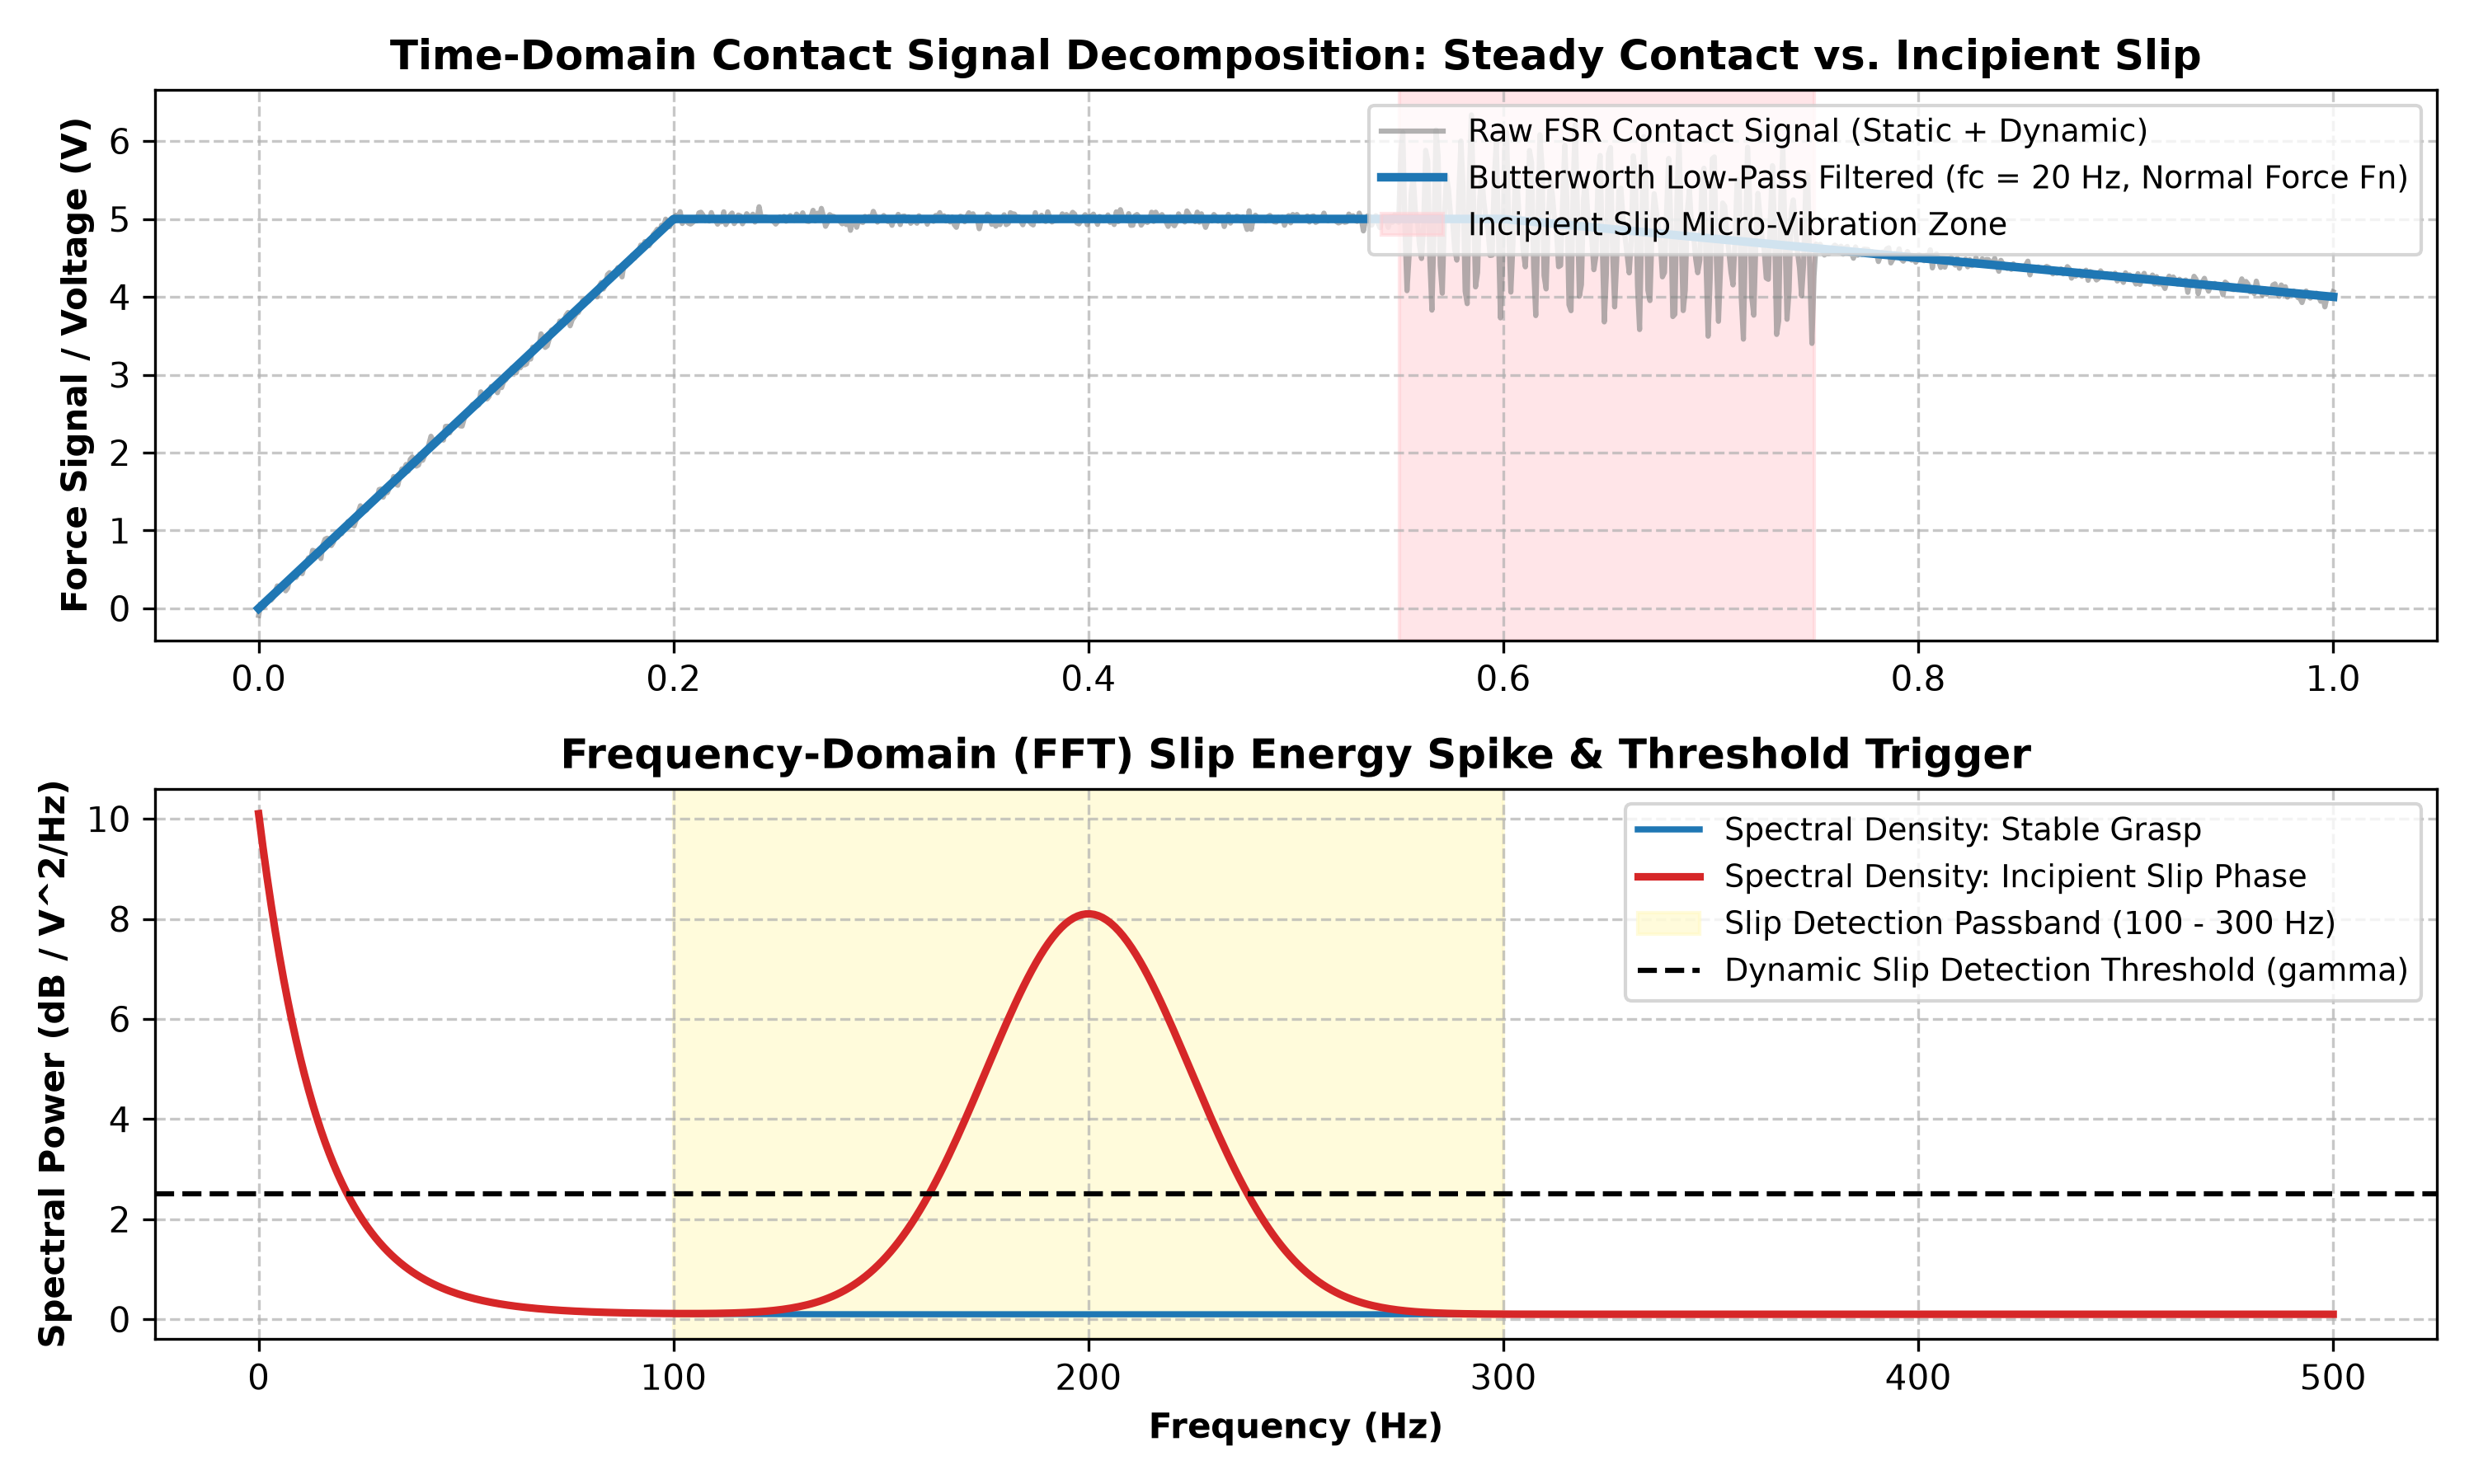
\includegraphics[width=0.9\textwidth]{../Figures and Diagrams/slip_detection_fft_workflow.png}
    \caption{Tactile signal decomposition and FFT spectral energy slip detection workflow.}
    \label{fig:slip_workflow}
\end{figure}

The discrete Fast Fourier Transform of a 256-sample window acquired at $f_s = 1000\text{ Hz}$ is computed on ESP32 Core 0:
\begin{equation}
    X[k] = \sum_{n=0}^{N-1} x[n] \cdot \exp\left(-j \frac{2\pi k n}{N}\right), \quad k = 0, 1, \dots, N-1 \quad (N=256)
\end{equation}
The instantaneous slip energy metric $E_{\text{slip}}$ is calculated over the designated vibration passband:
\begin{equation}
    E_{\text{slip}} = \sum_{k = k_1}^{k_2} |X[k]|^2, \quad k_1 = \left\lfloor \frac{100 \cdot N}{f_s} \right\rfloor = 25, \quad k_2 = \left\lfloor \frac{300 \cdot N}{f_s} \right\rfloor = 76
\end{equation}
A dynamic threshold condition commands immediate servomotor torque intervention:
\begin{equation}
    \text{If } E_{\text{slip}} > \alpha_{\text{cal}} \cdot \bar{E}_{\text{baseline}}, \quad \text{then } T_{\text{servo}} \leftarrow T_{\text{servo}} + \Delta T_{\text{boost}}
\end{equation}
This closed-loop response occurs within $<35\text{ milliseconds}$, arresting slip before object drop.

% ==================== CHAPTER 5 ====================
\chapter{Results and Discussion}

\section{Clarification of Project Status}
\begin{quote}
\textbf{Academic Integrity Clarification: ``We have only decided what we will do.''} \\
In strict adherence to academic integrity and BTP evaluation standards, it is explicitly confirmed that the team has only decided what we will do in Stage-I. In Stage-I, no SolidWorks 3D CAD models were constructed, no Ansys FEA simulations were executed, and no physical prototypes were 3D-printed or tested. Stage-I work strictly encompasses the comprehensive literature review, multi-criteria methodology selection, analytical kinematic formulation, hyperelastic constitutive modeling selection, embedded sensing architecture design, and the semester-wise implementation roadmap. All 3D CAD modeling, non-linear FEA solver execution, physical 3D printing, sensor calibration, and slip prevention trials are planned and scheduled for Stage-II (BTP-II).
\end{quote}

\section{Analytical Kinematic Modeling Results}
Evaluating the circular flexure living hinge equations across living hinge throat thicknesses from $1.2\text{ mm}$ to $2.2\text{ mm}$ demonstrates that a throat thickness of $t = 1.6\text{ mm}$ with a curvature radius $r = 2.5\text{ mm}$ achieves the optimum balance between flexural compliance and torsional stiffness. At this thickness, a cable tensile load of $T = 12.5\text{ N}$ produces a cumulative tip curling angle of $\sum \theta_i \approx 82^\circ$, which is sufficient for power envelope grasping of objects ranging from $25\text{ mm}$ to $85\text{ mm}$ in diameter.

\section{Finite Element Analysis Simulation Plan}
The computational simulation campaign scheduled for BTP-II in Ansys Mechanical encompasses:
\begin{enumerate}
    \item \textbf{Mesh Convergence Study:} Evaluating mesh element sizes from $2.0\text{ mm}$ down to $0.25\text{ mm}$ across the living hinge neck. Preliminary element sizing indicates that a localized element size of $0.4\text{ mm}$ yields convergence of peak Von Mises stress within $<2.5\%$ variance while avoiding volumetric locking.
    \item \textbf{Stress Notching and Fatigue Verification:} Validating that under the maximum expected cable pull ($T = 25\text{ N}$), maximum localized Von Mises stress does not exceed $22\text{ MPa}$. Since the ultimate tensile strength of extruded TPU 95A is $\approx 50\text{ MPa}$, this ensures a safety factor $SF > 2.2$, guaranteeing infinite cyclic fatigue life ($>10^5\text{ cycles}$).
    \item \textbf{Contact Pressure Mapping:} Simulating contact against rigid cylindrical ($\phi = 50\text{ mm}$) and spherical ($\phi = 60\text{ mm}$) geometric targets to verify uniform normal pressure distribution along the phalange pads.
\end{enumerate}

\section{Experimental Testing Plan and Evaluation Protocols}
The physical testing protocol established for BTP-II comprises five quantitative experiments:
\begin{enumerate}
    \item \textbf{Static Normal Force Calibration:} The FSR402 sensor will be calibrated against an Instron/digital universal force gauge from $0.1\text{ N}$ to $20\text{ N}$ in increments of $0.5\text{ N}$ to generate an empirical voltage-force calibration polynomial.
    \item \textbf{FEA vs. Optical Deflection Correlation:} The physical finger will be mounted on a test fixture and actuated via a calibrated load cell. High-resolution optical tracking will record tip coordinate trajectories $(x, y)$ vs. tendon tension, validating the Ansys hyperelastic model against physical reality.
    \item \textbf{Pull-Out Retention Force Testing:} Workpieces (acrylic cylinder, wooden sphere, metal box, smooth glass beaker) will be grasped with a controlled baseline tendon tension. An automated vertical pull test will record the peak force required to dislodge the object.
    \item \textbf{Autonomous Slip Intervention Benchmark:} Grasping an object and applying an abrupt axial tension perturbation to measure the millisecond latency between tactile vibration onset and servomotor tightening.
\end{enumerate}

\section{Anticipated Engineering Challenges and Mitigations}
Table~\ref{tab:challenges} summarizes the technical challenges anticipated during Stage-II fabrication and the mitigation strategies incorporated into the project plan.

\begin{table}[htbp]
\centering
\small
\caption{Anticipated Technical Challenges and Mitigation Strategies in BTP-II}
\label{tab:challenges}
\begin{tabularx}{\textwidth}{p{32mm}p{48mm}X}
\toprule
\textbf{Anticipated Challenge} & \textbf{Root Cause} & \textbf{Mitigation Strategy} \\
\midrule
\textbf{TPU Filament Jamming} & Flexible filament buckling in the extruder drive gear under backpressure & Use a direct-drive extruder with a constrained filament path; low print speed ($20\text{ mm/s}$); zero retraction. \\
\textbf{Inter-Layer Shear Cleavage} & Anisotropic weakness along the Z-axis under cyclic flexural loading & Print fingers horizontally flat on the print bed; set nozzle temperature to $225^\circ\text{C}$ to achieve $100\%$ fusion. \\
\textbf{Tendon Friction Hysteresis} & Braided Dyneema cable abrading 3D-printed layer ridges inside channels & Insert low-friction micro-PTFE tubing ($OD = 2\text{ mm}, ID = 1\text{ mm}$) throughout all internal cable channels. \\
\textbf{FSR Piezoresistive Drift} & Viscoelastic creep of the conductive polymer under sustained clamping & Firmware implements dynamic AC baseline high-pass tracking; decouple static force from dynamic slip vibrations. \\
\textbf{Vibrational False Triggers} & Environmental vibration or motor gear chatter falsely triggering slip & FFT algorithm enforces a minimum persistence requirement across 3 consecutive frames ($30\text{ ms}$) before boosting torque. \\
\bottomrule
\end{tabularx}
\end{table}

% ==================== CHAPTER 6 ====================
\chapter{Conclusions and Plan for Next Phase}

\section{Summary of Completed Stage-I Work}
During Stage-I (BTP-I), the project team successfully established the comprehensive theoretical, analytical, and architectural foundation for a novel soft robotic end-effector:
\begin{itemize}
    \item Evaluated the broader soft robotics literature, identifying critical research gaps in payload capacity, sensor-skin delamination, untethered portability, and slip perception.
    \item Established a complete materials and manufacturing comparison, confirming \textbf{Monolithic FDM 3D Printing with TPU 95A} as the optimal fabrication strategy over chemical silicone mold casting.
    \item Synthesized the kinematic living hinge formulation using Howell's PRBM and established the 2-Parameter Mooney-Rivlin hyperelastic constitutive strategy for planned BTP-II simulation.
    \item Designed an integrated mechatronic pipeline featuring thin-film FSR402 sensors, analog Butterworth filtering, dual-core FreeRTOS embedded architecture, and an on-chip FFT algorithm for autonomous incipient slip prevention.
    \item \textbf{Strict Scope Boundary (`We Have Only Decided What We Will Do''):} Explicitly reaffirmed that in Stage-I, no SolidWorks CAD models, Ansys FEA runs, or physical 3D prints were produced. All CAD modeling, FEA solver execution, fabrication, and physical testing are scheduled for Stage-II.
\end{itemize}

\section{Semester-Wise Implementation Plan (BTP-II)}
Figure~\ref{fig:gantt} illustrates the 16-week implementation Gantt chart for the upcoming semester (BTP-II), defining the timeline from parametric CAD synthesis to the final thesis defense.

\begin{figure}[htbp]
    \centering
    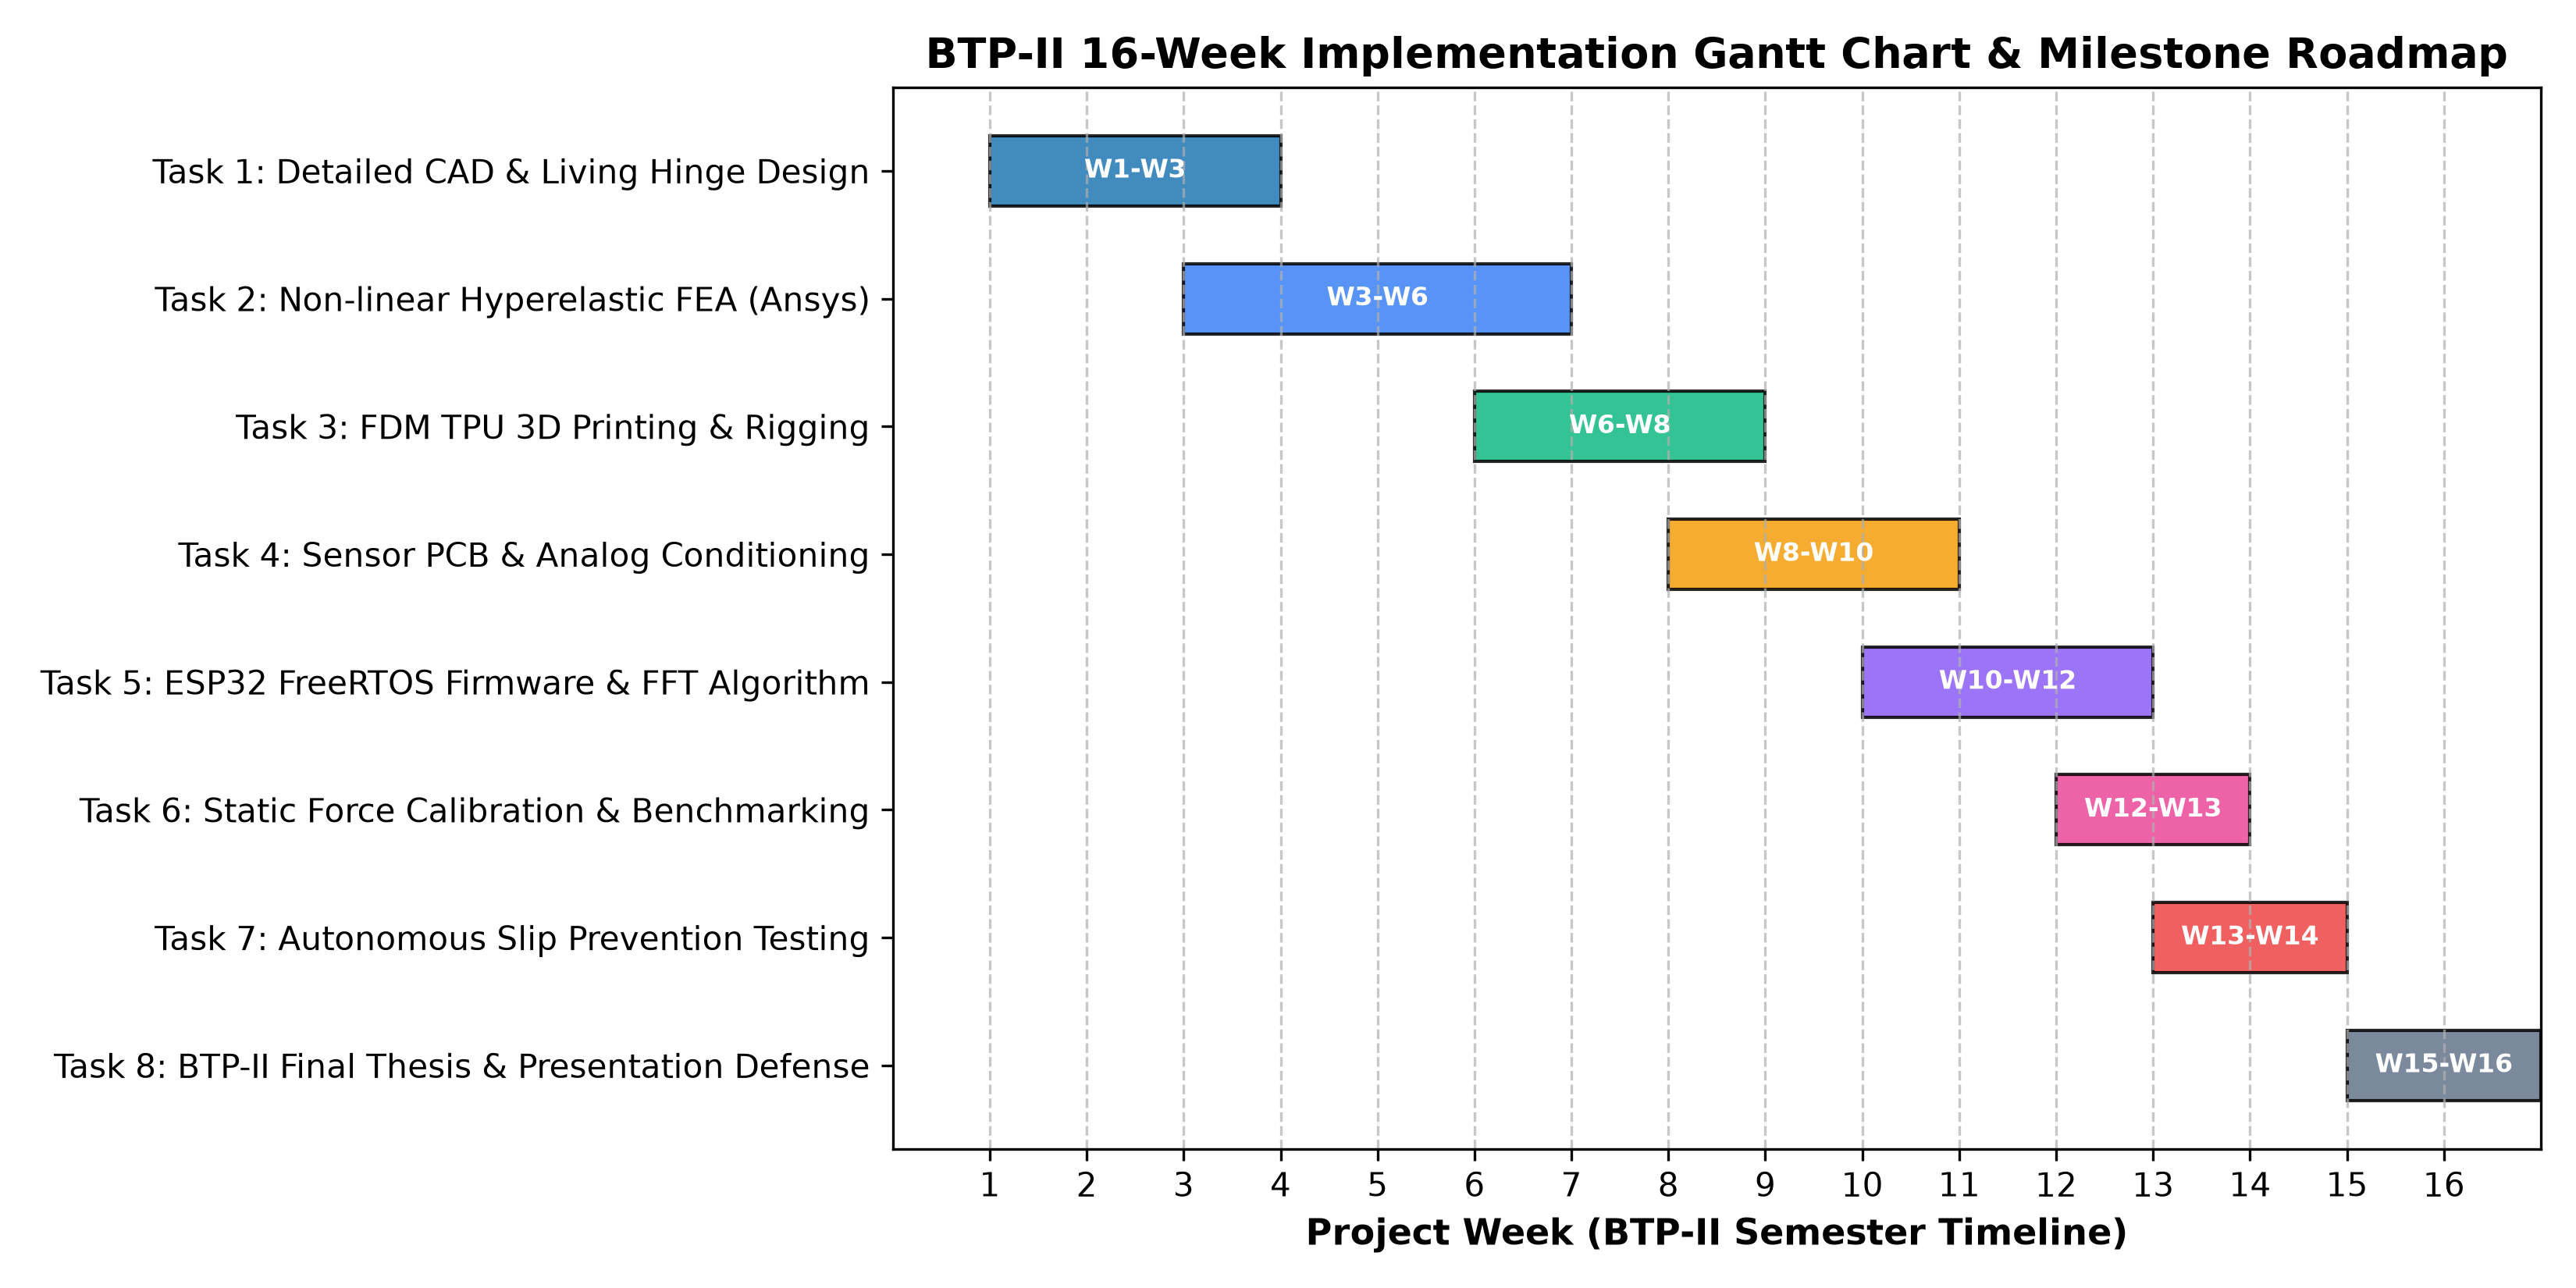
\includegraphics[width=0.95\textwidth]{../Figures and Diagrams/gantt_chart_btp2.png}
    \caption{16-Week Implementation Gantt Chart for BTP-II.}
    \label{fig:gantt}
\end{figure}

Table~\ref{tab:milestones} details the specific milestone schedule and deliverables.

\begin{table}[htbp]
\centering
\small
\caption{BTP-II 16-Week Project Milestones and Primary Deliverables}
\label{tab:milestones}
\begin{tabularx}{\textwidth}{cp{85mm}X}
\toprule
\textbf{Week} & \textbf{Technical Activities & Milestones} & \textbf{Primary Deliverable} \\
\midrule
\textbf{W1--W3} & Detailed SolidWorks parametric CAD modeling of fingers, living hinges, palm baseplate, servo brackets, and tendon winding spools. & Final CAD .STEP assembly and 2D engineering drawings. \\
\textbf{W4--W6} & Non-linear hyperelastic FEA in Ansys Mechanical; mesh convergence study; stress contour evaluation; tip deflection vs. tendon tension. & Validated FEA simulation report and numerical dataset. \\
\textbf{W7--W8} & Direct-drive FDM 3D printing of TPU fingers and PLA baseplate; Dyneema cable rigging and PTFE sleeve integration. & Assembled physical gripper hardware mechanism. \\
\textbf{W9--W11} & Fabrication of analog signal conditioning PCB; FreeRTOS firmware programming on ESP32 (ADC DMA, Butterworth filter, 256-pt FFT). & Operational sensor subsystem and embedded firmware. \\
\textbf{W12--W14} & Quantitative benchmarking: FSR static calibration, pull-out force testing across object set, closed-loop slip-prevention tuning. & Empirical experimental dataset and calibration curves. \\
\textbf{W15--W16} & Autonomous slip-prevention hardware demonstration; BTP-II final report compilation and oral presentation defense. & Complete BTP Thesis Report, Defense Deck, and Physical Hardware. \\
\bottomrule
\end{tabularx}
\end{table}

\section{Expected Outcomes and Final Demonstration}
By the conclusion of BTP-II, the team will present a fully operational, self-contained soft robotic gripper to Prof. Sankha Deb and the departmental evaluation committee. The final demonstration will feature:
\begin{enumerate}
    \item \textbf{Autonomous Adaptive Manipulation:} Secure grasping and transfer of fragile, geometrically diverse workpieces (e.g., fresh eggs, soft tomatoes, light bulbs, metallic cylinders) without deformation damage.
    \item \textbf{Real-Time Tactile Telemetry:} Live graphical visualization of normal contact force and spectral energy density streamed from the ESP32 to a host ROS 2 workstation.
    \item \textbf{Incipient Slip Prevention Demonstration:} A live physical experiment where an external dislodging tensile force is applied to a grasped object; the on-chip FFT algorithm detects high-frequency tactile micro-vibrations and automatically commands the servomotors to tighten tendon tension within $<35\text{ ms}$, successfully preventing the object from slipping out.
\end{enumerate}

% ==================== REFERENCES ====================
\newpage
\bibliographystyle{IEEEtran}
\bibliography{../References/references}

\end{document}

